% --------------------------------- Familia  eliptica
\subseccion{Familia eliptica}
\label{Ssec:MP:FamiliaEliptica}


% --------------------------------- Familia  eliptica real

\subsubseccion{Caso real}
\label{Ssec:MP:FamiliaElipticaReal}

% --------------------
% Bilingsley p. 
% Kay p.
% Lehman & Casela p. 
% Kotz & Balakrishnan p.
% Robert p.
% van den Bos p.
% Cencov p.
% Ibarola Perez p.
% Mukhopadhyay p.

El estudio de  estos vectores es bastante antigua. Hace  falta volver a trabajos
de Maxwell en 1867  sobre la teoria del gas para encontrar  unas de las primeras
menciones  a este  formalismo~\cite{Max67}  o~\cite[pp.~377--391]{Nie52:v1}.  El
problema de Maxwell era de encontrar una distribuci\'on (tridimensional) que sea
isotropica  y  separable   a  la  vez:  monstr\'o  que   tal  distribuci\'on  es
necesariamente    gausiana    (es     ahora    conocido    como    teorema    de
Maxwell-Hershel~\footnote{Ver~\cite[Prop.~4.11]{BilBre99}.   Se notar\'a  que no
  hay muchas menciones  de este teorema bajo esta  denominaci\'on. no sabemos si
  la raz\'on es que  no tienen ni Maxwell, ni Herschel la  partenidad o si no lo
  revendicaron. Sin embargo, ver~\cite{Max67}}.   Volveremos en este teorema. La
clase de  las distribuciones  eliptical, o a  simetr\'ia eliptica  fue estudiada
intensivamente  formalmente~\cite{Bar34,  Bar34:07,  Ver64, McgWag68,  CamHua81,
  Eat81,  Kan94,  Lau75,  Yao73,   KotNad01,  FanKot90,  Mui82,  BilBre99}.  Fue
tambi\'en  usadas   en  aplicaciones  en   estad\'istica~\cite{BlaTho68,  Chu73,
  YanKot03,  ArePin06,  BauPas07,  ChiPas08},   o  procesamiento  de  se\~nal  o
imagenes~\cite{Gol76, RanWei93, RanWei95, ZozVig10, Zoz12}, entre otros.

Empezamos  por  la  definici\'on,  antes  de  ir  m\'as  all\'a  estudiando  sus
propiedades remarcables.

\begin{definicion}[Vector esfericamente invariante]
  Sea  \  $X$  \  vector   aleatorio  $d$-dimensional  real.   $X$  \  es  dicho
  esfericamente  invariante,  o   rotacionalmente  invariante,  o  a  simetr\'ia
  esferica, o de distribuci\'on esferica \ si para cualquier matriz ortogonal (o
  de rotaci\'on)~\footnote{Recordarse que \ $O$  \ es ortogonal o de rotaci\'on
    si \ $O O^t = O^t O = I$.} \ $O$,
  %
  \[
  O  X  \: \egald  \: X
  \]
  %
\end{definicion}

Tales vectores modelizan naturalmente  fenomenos isotropicos. Pero m\'as all\'a,
se puede que haya direcciones  privilegiadas ortogonales pero con simetrias, \ie
en  lugar  de   simetr\'ias  esfericas,  simetr\'ias  como  en   una  pelota  de
rugby. Adem\'as, se puede que eso se pasa al torno de un punto no cero.
%
\begin{definicion}[Vector a simetr\'ia eliptica]
  Sea  \  $X$  \ vector  aleatorio  $d$-dimensional  real.   $X$  \ es  dicho  a
  simetr\'ia  eliptica,   o  elipticalmente  invariante,   o  de  distribuci\'on
  eliptica, al torno de \ $m \in  \Rset^d$, \ si existe una matriz \ $\Sigma \in
  P_d^+(\Rset)$ \ tal que para cualquier matriz ortogonal \ $O$,
  %
  \[
  O  \,   \Delta^{-\frac12}  \,  Q^t  \left(   X  -  m  \right)   \:  \egald  \:
  \Delta^{-\frac12} \, Q^t \left( X - m \right)
  \]
  %
  donde la  matriz diagonal \ $\Delta > 0$ \ es  la matriz de  autovalores de \
  $\Sigma$ \  y \ $Q$ \  la matriz de los  autovectores correspondientes (matriz
  ortogonal~\cite{Bha97, Bha07, HorJoh13}), \ $\Sigma  = Q \Delta Q^t$. Dicho de
  otra manera, \ $\Delta^{-\frac12} Q^t \left(  X - m \right)$ \ es a simetr\'ia
  esferica.

  $m$ \ es llamado {\em par\'ametro de posici\'on} y \ la matriz \ $\Sigma$ \ es
  llamada {\em matriz caracter\'istica}.
\end{definicion}
%
Se puede inmediatamente  ver que \ $\Sigma$ \ es definida  por lo menos mediante
un factor escalar. De hecho, si un \ $\Sigma$ \ conviene, cualquier \ $a \Sigma$
\ con \ $a > 0$ \ conviene tambi\'en.

Comparativamente a un  vector esfericamente invariante, \ $m$ \  es el centro de
simetr\'ia,   $P$   contiene   las   direciones   de   ``estiramientos''   y   \
$\Delta^{\frac12}$  \   los  factores  de   estiramientos,  $X  \egald  m   +  P
\Delta^{\frac12} Y$ \  con \ $Y$ \ a simetr\'ia  esferica. Para \ $m =  0$ \ y \
$\Delta \propto I$, se recupera obviamente un vector a simetr\'ia esferica.

Como lo hemos visto, un vector aleatorio es completamente definido por su medida
de  probabilidad,  o  equivalentemente  por su  funci\'on  car\'acteristica.  La
\'ultima tiene una forma particular en el contexto eliptico:
%
\begin{teorema}[Funci\'ones y generadoras caracter\'isticas]\label{Teo:MP:GeneradorasCaracteristicas}
%
  Sea \ $X$ \ vector aleatorio $d$-dimensional a simetr\'ia eliptica al torno de
  \   $m  \in  \Rset^d$   \  y   de  matriz   caracter\'istica  \   $\Sigma  \in
  P_d^+(\Rset)$. Entonces la funci\'on caract\'eristica se escribe bajo la forma
  %
  \[
  \Phi_X(\omega)  = e^{\imath  \,  \omega^t m}  \varphi_X\left( \omega^t  \Sigma
    \omega \right)
  \]
  %
  donde  \  $\varphi_X:  \Rset_+  \mapsto  [-1 \; 1]$ \  escalar,  es  llamado  {\em
    generadora  caracter\'istica}. Tomando el  logaritmo, obviamente  la secunda
  funci\'on caracteristica se escribe
  %
  \[
  \Psi_X(\omega) =  \imath \, \omega^t  m + \psi_X\left( \omega^t  \Sigma \omega
  \right)
  \]
  %
  donde  \ $\psi_X  =  \log \varphi_X:  \Rset_+  \mapsto \Cset$  \ escalar.   La
  llamaremos  {\em secunda generadora  caracter\'istica}. Reciprocamente,  si la
  funci\'on caracter\'istica tiene esta forma, \ $X$ \ es a simetr\'ia eliptica.
\end{teorema}
%
\begin{proof}
  Sea \  $Y = \Delta^{-\frac12} Q^t  \left( X - m  \right)$ \ con \  $\Sigma = Q
  \Delta  Q^t$  \ diagonalizaci\'on  de  \  $\Sigma$.   Por definici\'on  y  del
  teorema~\ref{Teo:MP:PropiedadesFuncionCaracteristica},  por  cualquier  matriz
  ortogonal \ $O$ \ y cualquier \ $\omega \in \Rset^d$
  %
  \[
  \Phi_Y(\omega) = \Phi_{O Y}(\omega) = \Phi_Y(O^t \omega)
  \]
  %
  En  otros  terminos,  la  funci\'on  caracter\'istica  queda  invariante  bajo
  cualquier transformaci\'on  ortogonal (rotaci\'on) sobre  $\omega$, y entonces
  depende solamente de  la norma euclideana de \ $\omega$.  Es decir, existe una
  funci\'on escalar \ $\varphi_X$ \ tal que
  %
  \[
  \Phi_Y(\omega) = \varphi_X(\omega^t \omega)
  \]
  %
  De nuevo, del teorema~\ref{Teo:MP:PropiedadesFuncionCaracteristica},
  %
  \[
  \Phi_X(\omega)  \:  = \:  \Phi_{Q  \Delta^{\frac12} Y  +  m}(\omega)  \: =  \:
  e^{\imath  \, \omega^t  m} \,  \Phi_Y( \Delta^{\frac12}  Q^t \omega)  \:  = \:
  e^{\imath \, \omega^t m} \, \varphi_x( \omega^t Q \Delta Q^t \omega)
  \]
  % 
  lo que  cierra la prueba  directa. Reciproca, si  \ $\Phi_X$ \ tiene  la forma
  dada, para  cualquier matriz ortogonal \  $O$ \ $\Phi_{O  Y}(\omega) = \Phi_Y(
  O^t \omega ) = \Phi_Y(\omega)$ \  y, por relaci\'on uno-uno entre la medida de
  probabilidad  de una variable  aleatorio y  su funci\'on  caracter\'istica, $Y
  \egald O Y$.

  Al final, de la simetr\'ia herm\'itica  de la funci\'on de repartici\'on, y de
  la simetr\'ia  eliptica, tenemos $\varphi_X^*\left(  \| \omega \|^2  \right) =
  \varphi_X\left(  \| -\omega  \|^2  \right) =  \varphi_X\left(  \| \omega  \|^2
  \right)$,  lo que proba  que \  $\varphi_X$ \  es a  valores reales,  siendo a
  valores tambi\'en de modulo menor que $\varphi_X(0) = 1$.
\end{proof}
%
Se notar\'a que si tomamos  una matriz caracter\'istica $\Sigma$ y la generadora
correspondiente  $\varphi$, \  $a  \Sigma$ \  y  \ $\varphi_X\left(  \frac{u}{a}
\right)$ \ conviene tambi\'en, lo que  es de acuerdo con la indeterminencia de \
$\Sigma$ \ bajo un factor positivo.  Se puede a\~nadir un v\'inculo, por ejemplo
fijando  \  $\Tr \Sigma$  \  para  que  \ $\Sigma$  \  y  \ $\varphi_X$  \  sean
\'unicamente definidas. Entonces, \ $X$ \ ser\'a completamente caracterizado por
\ $m, \: \Sigma$ \ y \ $\varphi_X$, y escribiremos
%
\[
X \, \sim \, \ED \left( m , \Sigma , \varphi_X \right)
\]
%
y   los  conjuntos  de   generadoras  caracter\'isticas   que  resultan   de  la
restricci\'on  de   $\PD_d$  (y  de  $\PD$)  a   las  funciones  caracteristicas
esfericamente invariante como
%
\[
\PDSI_d = \big\{ 
%\begin{array}{lll} 
\varphi: \Rset_+ \mapsto [-1 ; 1]  \:\: \mbox{  continuas con } \:\: \varphi(0) = 1  \tq \Phi: 
%& \Rset^d \to \Cset & \in \PD_d \\[-1mm] & 
x \mapsto \varphi\left( \| x \|^2 \right)
% & \end{array} 
\in \PD_d \big\}
\]
%
y
%
\[
\PDSI = \bigcap_{d=1}^{+\infty} \PDSI_d = \big\{ 
%\begin{array}{lll} 
\varphi: \Rset_+ \mapsto [-1 ; 1]  \:\: \mbox{  continuas con } \:\: \varphi(0) = 1  \tq \Phi: 
%& \Rset^d \to \Cset & \in \PD_d \\[-1mm] & 
x \mapsto \varphi\left( \| x \|^2 \right)
% & \end{array} 
\in \PD \big\}
\]
%
(ver notaciones).

Vamos a  ver m\'as adelante varios  ejemplos de variable  a simetr\'ia elipticas
que ya hemos vistos en las subsecciones anteriores.  Un caso particular que va a
jugar un rol  importante es el de un vector de  distribuci\'on uniforme sobre la
esfera \ $\Sset_d$, \ $U \sim \U(\Sset_d)$~\cite{FanKot90}:
%
\begin{ejemplo}[Distribuci\'on uniforme sobre la esfera unitaria]\label{Ej:MP:GeneCaracUniformeEsfera}
%
  Sea \  $U \sim \U(\Sset_d)$. Entonces  \ $U \sim  \ED\left( 0 , I  , \varphi_U
  \right)$ \ con
  %
  \[
  \varphi_U(u)   =  2^{\frac{d}{2}-1}   \Gamma\left(   \frac{d}{2}  \right)   \,
  u^{-\frac{d-2}{4}} \, J_{\frac{d}{2}-1}\left( \sqrt{u} \right)
  \]
  %
  con \ $J_\nu$ \ funci\'on de Bessel~\footnote{Seg\'un Sch{\oe}nberg~\cite[Nota
    de  pie~9]{Sch38} and Watson~\cite[p.~24,  nota de  pie~*]{Wat22}, deber\'ia
    llamarse  integral  de  Poisson  proque fue  introducida  primariamente  por
    Poisson en 1823~\cite{Poi23}, pero  apareci\'o implicitamente a\'un antes en
    trabajos  de Euler~\cite[Cap.~X, \S~1036]{Eul1769}.}   primera especie  y de
  orden $\nu$ (ver notaciones).
  
  De hecho, de la definici\'on de la funci\'on caracter\'istica, tenemos
  %
  \[
  \Phi_U(\omega) =  \frac{1}{|\Sset_d|} \int_{\Sset_d} e^{\imath  \, \omega^t s}
  d\mu_H(s)
  \]
  %
  con \ $\mu_H$ \ la medida de Haar~\footnote{Para \ $S \subset \Sset$ \ $\mu(S)
    =    |S|$.}     sobre    la    esfera    y   \    $|\Sset_d|    =    \frac{2
    \pi^{\frac{d}{2}}}{\Gamma\left(  \frac{d}{2} \right)}$  \ la  surfaca  de la
  esfera  unitaria~\cite{GraRyz15}.   Ahora,  denotanto  \  $\Sset_d^+$  \  y  \
  $\Sset_d^-$  \ respectivamente  la semiesfera  superior y  inferior,  se puede
  parametrizar \  $s \in \Sset_d^{\pm}$ \  bajo la forma \  $s = \begin{bmatrix}
    b^t & \pm \sqrt{1-\|b\|^2} \end{bmatrix}^t, \quad b \in \Bset_{d-1}$, lo que
  da,  siguiendo~\cite[ec.~4.644]{GraRyz15}  (cambio  de  variables)  y  notando
  $\mu_L$ \ la medida de Lebesgue,
  %
  \begin{eqnarray*}
  \Phi_U(\omega) & = & \frac{2 \, \Gamma\left( \frac{d}{2}
  \right)}{\pi^{\frac{d}{2}}} \int_{\Bset_{d-1}} \frac{e^{\imath \, \omega^t
  s}}{\sqrt{1-\|b\|^2}} d\mu_L(b)\\[2mm]
  %
  & = & \frac{\Gamma\left( \frac{d}{2} \right)}{\sqrt{\pi} \, \Gamma\left(
  \frac{d-1}{2} \right)} \int_0^{\pi} e^{\imath \, \| \omega \| \cos\theta} \,
  \sin^{d-2}\theta \, d\theta
  \end{eqnarray*}
  %
  Al final,  de la forma de la  funci\'on de Bessel~\cite[Ec.~8.411-7]{GraRyz15}
  (ver tambi\'en~\cite{AbrSte70, Wat22, GraMat95}), se obtiene
  %
  \[
  \Phi_U(\omega) =  \frac{2^{\frac{d}{2}-1} \Gamma\left( \frac{d}{2} \right)}{\|
    \omega \|^{\frac{d}{2}-1}} \, J_{\frac{d}{2}-1}\left( \|\omega\| \right)
  \]
  %
  lo que cierra  la prueba. Volveremos a esta  funci\'on caracteristica tratando
  de las coordenadas esfericas.
\end{ejemplo}

La forma de la funci\'on caracter\'istica tiene varias consecuencias. La primera
es  que se  puede escribir  estocaticamente un  vector a  simetr\'ia  eliptica a
partir de un vector esfericamente invariante de varias maneras, entre otros:
%
\begin{corolario}
  Sea  \ $Y  \sim  \ED(0,I,\varphi_Y)$, \  $m \in  \Rset^d$  \ y  \ $\Sigma  \in
  P_d^+(\Rset)$. \ Sean \ $\Sigma = Q \Delta Q^t$ \ la descomposici\'on diagonal
  de \ $\Sigma$, \ $\Sigma^{\frac12} = Q \Delta^{\frac12} Q^t$ \'unica matriz de
  \  $P_d^+(\Rset)$ \  raiz cuadrada  de \  $\Sigma$,  y \  $\Sigma =  L L^t$  \
  descomposici\'on  de  Cholesky   de  \  $\Sigma$,  con  \   $L$  \  triangular
  inferior~\cite{HorJoh13, Bha07}.  Entonces
  %
  \[
  Q \Delta^{\frac12} Y + m \: \egald \:  \Sigma^{\frac12} Y + m \: \egald \: L Y
  + m \: \sim \: \ED(m,\Sigma,\varphi_Y)
  \]
\end{corolario}
%
\begin{proof}
  El             resultado            es             consecuencia            del
  teorema~\ref{Teo:MP:PropiedadesFuncionCaracteristica}  y  de  la forma  de  la
  funci\'on caracter\'istica del teorema~\ref{Teo:MP:GeneradorasCaracteristicas}.
\end{proof}

Una otra consecuencia es que, dado el orden, el tensor de los momentos tiene una
structura dada para cualquier ley, bajo un factor escalar que depende de la ley.
Eso vale tambi\'en para los cumulantes:
%
\begin{teorema}[Momentos centrales y cumulantes]\label{Teo:MP:MomentosCumulantesEliptica}
%
  Sea \  $X$ \  vector aleatorio $d$-dimensional  de distribuci\'on  eliptica al
  torno  de  un  vector \  $m$,  y  de  matriz  caracter\'istica \  $\Sigma  \in
  P_d^+(\Rset)$.  Entonces, si  estos momentos y cumulantes existen,  \ $m$ \ es
  la media de \ $X$, \ie
  %
  \[
  \zeta_1[X] = 0, \qquad \kappa_1[X] = m
  \]
  %
  y para cualquier orden superior a  $2$, los momentos centrales y cumulantes de
  orden impares son ceros,
  %
  \[
  \zeta_{2 k + 1}[X] = \kappa_{2 k + 1}[X] = 0, \qquad k \ge 1
  %_{i_1,\ldots,i_{2  k  +1}}[X] =  \kappa_{i_1,\ldots,i_{2  k  +1}}[X] =  0,
  %\qquad k \ge 1
  \]
  %
  y los de orden pare son dados para \ $k \ge 1$, por
  %
  \[
  \zeta_{2 k}[X] = \alpha_k\left(  \varphi_X   \right) \T_k(\Sigma)
  %{i_1,\ldots,i_{2   k}}[X]   =   \alpha_k\left(  \varphi_X   \right)   \,
  %\psi_{i_1,\ldots,i_{2 k}}(\Sigma)
 \qquad  y \qquad \kappa_{2 k}[X] = \alpha_k\left(  \psi_X   \right) \T_k(\Sigma)
%_{i_1,\ldots,i_{2 k}}[X]
%  = \alpha_k\left( \psi_X \right) \, \psi_{i_1,\ldots,i_{2 k}}(\Sigma)
  % (-2)^k \, \varphi_X^{(k)}(0)  \sum_{\pi \in \Pi_{2 k ,  2}} \prod_{(l,n) \in
  %   \pi} \Sigma_{i_l,i_n}
  \]
  %
  % y
  %  %
  % \[
  %  \kappa_{i_1,\ldots,i_{2 k}}[X]  = (-2)^k  \, \psi_X^{(k)}(0)  \sum_{\pi \in
  %   \Pi_{2 k , 2}} \prod_{(l,n) \in \pi} \Sigma_{i_l,i_n}
  % \]
  %
  con el coefficient \ $\alpha_k$ \ dado por
  %
  \[
  \alpha_k(f) = (-2)^k f^{(k)}(0)
  \]
  %
  y el tensor \ $\T_k(\Sigma)$ \ de orden \ $2 k$ \ de componentes
  %
  \[
  \T_{i_1,\ldots,i_{2k}}(\Sigma) = \sum_{\pi \in \Pi_{2 k , 2}} \prod_{(l,n) \in
    \pi} \Sigma_{i_l,i_n}
  % \qquad \mbox{y} \qquad \alpha_k(f) = (-2)^k f^{(k)}(0)
  \]
  %
  donde   \  $\Pi_{2   k  ,   2}$   \  es   el  conjunto   de  particiones   por
  pares~\footnote{Por  ejemplo, $\Pi_{4,2}  =  \Big\{ \big\{  \{1,2\} ,  \{3,4\}
    \big\} \:  , \: \big\{  \{1,3\} ,  \{2,4\} \big\} \:  , \: \big\{  \{1,4\} ,
    \{2,3\} \big\} \big\}$; cuando \ $\pi = \big\{ \{1,3\} , \{2,4\} \Big\}$, el
    t\'ermino del producto es \ $\Sigma_{i_1,i_3} \Sigma_{i_2,i_4}$.} de $\{ 1 ,
  \ldots , 2 k \}$.
\end{teorema}
%
Una prueba  es dada  por inducci\'on en~\cite{BerBen86}  para los  momentos (ver
tambi\'en~\cite[p.~44]{FanKot90} para el resultat  con los momentos).  Damos una
prueba m\'as directa, valida para ambos momentos y cumulantes.
%
\begin{proof}
  Recordamosnos que para \ $k \in \Nset^*, \quad (i_1 , \ldots , i_k) \in \{ 1 ,
  \ldots , d \}^k$,
  %
  \[
  \zeta_{i_1,\ldots,i_k}[X]     =     (-    \imath)^k     \left.\frac{\partial^k
      \Phi_{X-m_X}}{\partial          \omega_{i_1}          \cdots          \partial
      \omega_{i_k}}\right|_{\omega=0}       \qquad       \mbox{y}       \qquad
  \kappa_{i_1,\ldots,i_k}[X]     =    (-     \imath)^k    \left.\frac{\partial^k
      \Psi_X}{\partial          \omega_{i_1}          \cdots          \partial
      \omega_{i_k}}\right|_{\omega=0}
  \]
  
  Por  definici\'on  de  los  momentos  centrales  $\zeta_1  =  0$.   Luego,  de
  $\Psi_X(\omega)  =  \imath \,  \omega^t  m  +  \log\left( \varphi_X(  \omega^t
    \omega) \right)$ \ tenemos
  %
  \[
  \nabla_\omega \Psi_X(\omega) =  \imath \, m + \frac{2  \, \varphi_X'( \omega^t
    \omega)}{\varphi_X'( \omega^t \omega)} \, \omega
  \]
  %
  Recordandose que \ $\Phi_X(0) = \Esp\left[  e^{\imath \, 0^t X} \right] = 1$ \
  y \ $m =  - \imath \, \nabla_\omega \Psi_X(0)$: \ $m$ \ es  la media de \ $X$\
  lo que corresponde a la intuici\'on.

  Luego, salimos de  la formula de Hardy, extensi\'on de de  Fa\`a di Bruno, que
  vimos  secci\'on~\ref{Ssec:MP:GeneradoraCumulantes}  que  recordamos:  Para  \
  $h(\omega) = f\left( g(\omega) \right),  \quad \forall \: n \in \Nset^*, \quad
  \forall \: (i_1 , \ldots , i_n ) \in \{ 1 , \ldots , d \}^n$,
  %
  \[
  \frac{\partial^n  h}{\partial  \omega_{i_1}  \cdots \partial  \omega_{i_n}}  =
  \sum_{\pi  \in \Pi_n}  f^{(|\pi|)}\left( g(\omega)  \right) \prod_{B  \in \pi}
  \frac{\partial^{|B|} g}{\displaystyle \prod_{j \in B} \partial \omega_{i_j}}
  \]
  %
  con \ $\Pi_n$  \ el conjunto de las  particiones de \ $\{ 1  , \ldots , n
  \}$ \ y \ $f^{(l)}$  la $l$-esima  derivada  de $f$.   En  la  expresi\'on de  los
  momentos centrales y cumulantes tenemos
  %
  \[
  g(\omega) = \sum_{i,j=1}^d \omega_i \omega_j \Sigma_{i,j}
  \]
  %
  as\'i que, por simetr\'ia de $\Sigma$,
  %
  \[
  \frac{\partial  g}{\partial   \omega_{j_1}}  =  2   \sum_{l=1}^d  \omega_{j_1}
  \Sigma_{j_1,l},  \qquad  \frac{\partial^2  g}{\partial  \omega_{j_1}  \partial
    \omega_{j_2}}  =  2 \Sigma_{j_1,j_2},  \qquad  \forall  \:  n \ge  3,  \quad
  \frac{\partial^n g}{\prod_{l=1}^n \partial \omega_{j_l}} = 0
  \]
  %
  Es decir que, para $n \ge 1$,
  %
  \[
  \left.      \frac{\partial^n    g}{\prod_{l=1}^n     \partial    \omega_{j_l}}
  \right|_{\omega = 0} = \left\{\begin{array}{ccl}
  %
  2   \Sigma_{j_1,j_2} & \mbox{si} & n = 2\\[2mm]
  %
  0 & \mbox{si} & n \ne 2
  %
  \end{array}\right.
  \]
  %
  Entonces,  en la formula  de Hardy  tomada en  $\omega =  0$ quedan  solas las
  particiones  que  contienen unicamente  pares  de  indices.   Eso da  momentos
  centrales y cumulantes nulos para $k$ impar (obvio por sim\'etria). Adema\'as,
  siendo \  $\Pi_{2 k , 2}$  \ el conjunto de  particiones por pares de  $\{ 1 ,
  \ldots , 2 k \}$, notando que necesariamente cada partici\'on de \ $\Pi_{2 k ,
    2}$ \ contiene \ $k$ \ pares,
  %
  \[
  \left.   \frac{\partial^{2  k}   h}{\partial   \omega_{i_1}  \cdots   \partial
      \omega_{i_{2  k}}}\right|_{\omega =  0} =  \sum_{\pi  \in \Pi_{2  k ,  2}}
  f^{(k)}(0) \prod_{(l,n) \in \pi} \left( 2 \Sigma_{i_l,i_n} \right)
  \]
  %
  La prueba  se cierra  tomando respectivamente  \ $f =  \varphi_X$ \  y \  $f =
  \psi_X$.
\end{proof}
%
Veremos m\'as adelante una prueba a\'un m\'as directa y obvia que, a orden dado,
el tensor  de los  momentos centrales  tiene una structura  dada bajo  un factor
escalar  dependiendo  de la  ley.   Lo  que es  menos  obvio,  de la  relaci\'on
momentos-cumulantes, que eso vale para el tensor de los cumulantes, y que, m\'as
que eso, estas structuras son las mismas.

De este  resultado se puede tambi\'en  explicitar la matriz de  covariancia y el
tensor curtosis para un vector a simetr\'ia eliptica~\cite[p.~44]{FanKot90}:
%
\begin{corolario}\label{Lem:MP:MediaCovarianzaEliptica}
  Sea \  $X$ \  vector aleatorio $d$-dimensional  de distribuci\'on  eliptica de
  matriz caracter\'istica \ $\Sigma \in P_d^+(\Rset)$. Entonces
  %
  \[
  \Sigma_X = - 2 \,  \varphi_X'(0) \, \Sigma
  \]
  %
  y
  %
  \[
  \kappa_X   =   \frac{\varphi_X''(0)}{4    \,   \big(   \varphi_X(0)   \big)^2}
  \sum_{i,j=1}^d \Big( \left( \un_i \un_i^t \right) \otimes \left( \un_j \un_j^t
  \right) + \left( \un_i \un_j^t  \right) \otimes \left( \un_i \un_j^t \right) +
  \left( \un_i \un_j^t \right) \otimes \left( \un_j \un_i^t \right) \Big)
  \]
  %
\end{corolario}
\begin{proof}
  El resultado es inmediato por lo  de la covarianza.  Para la curtosis, momento
  central de  orden cuatro del  vector normalizado, es equivalente  considerar \
  $\Sigma  = -  \frac{1}{2  \, \varphi_X(0)}  I$,  lo que  da  el resultado  del
  corrolario.
\end{proof}
%
Nota: de $\Tr(\Sigma_X) = \Tr\left( \Esp\left[ (X-m_X) (X-m_X)^t \right] \right)
= \Esp\left[ (X-m_X)^t  (X-m_X) \right]$ \ tenemos para  $U \sim \U(\Sset_d)$, \
$\Tr(\Sigma_U) = 1$, \ie
%
\[
\mbox{Para } \: U \sim \U(\Sset_d), \quad \Sigma_U = \frac{1}{d} I
\]
%Se  notar\'a  que  $\varphi_X(0)  =  1$  \  m\'axima,  y  que  necesariamente  \
%$\varphi_X'(0)  < 0$,  o, tambi\'en,  que $\varphi_X''(0)  > 0$:  $\phi_X$  \ es
%(localmente) concava al torno de $0$;

Se  puede  ver  de  este  corolario  que  la  covarianza  es  proporcional  a  \
$\Sigma$. Es decir que un v\'inculo que se puede poner tambi\'en para fijar \ $(
\Sigma , \varphi_X )$ \ es de  imponer un homotecia a \ $\varphi_X$ \ para tener
$\varphi_X'(0) = - \frac12$, para que \ $\Sigma$ \ y \ $\Sigma_X$ \ coincidan.

De  la  forma de  la  funci\'on caracter\'istica  se  proba  tambi\'en que  para
cualquier transformaci\'on  af\'in de un  vector a simetr\'ia eliptica  queda un
vector a simetr\'ia eliptica:
%
\begin{teorema}\label{Teo:MP:TranformacionAfinEliptica}
  Sea  \  $X \,  \sim  \,  \ED(m,\Sigma,\varphi_X)$  \ $d$-dimensional,  $A  \in
  \M_{d',d}(\Rset)$  \ de  rango  lleno tal  que  \ $d'  \le  d$ \  y  \ $c  \in
  \Rset^{d'}$. Entonces
  %
  \[
  A X + c \: \sim \: \ED(A m + c , A \Sigma A^t , \varphi_X)
  \]
  %
\end{teorema}
%
\begin{proof}
  El  resultado es  inmediato  de  la forma  de  la funci\'on  caracter\'istica,
  teorema~\ref{Teo:MP:GeneradorasCaracteristicas}   y   como  consecuencia   del
  teorema~\ref{Teo:MP:PropiedadesFuncionCaracteristica}.
\end{proof}
%
En particular, la proyecci\'on de  un vector a simetr\'ia eliptica queda eliptica
al  torno de  la proyecci\'on  del vector  posici\'on, con  la  misma generadora
caracter\'istica.
%
%\begin{definici\'on}
%  En lo que sigue, se notar\'a
%  %
%  \[
%
%  \]
%
%\end{definici\'on}

Eso  v\'incula   tambi\'n  un  vector  a  simetr\'ia   eliptica  con  cualquier
proyecci\'on:
%
\begin{teorema}[Proyecci\'on y componentes]\label{Teo:MP:ProyeccionComponentesEliptica}
  Sea \ $X$, vector aleatorio $d$-dimensonal de componentes $X_i$. Entonces
  %
  \[
  X \sim \ED(m,\Sigma,\varphi_X) \qquad  \Longleftrightarrow \qquad \forall \: a
  \in \Rset^d, \quad a^t (X - m) \egald \sqrt{\frac{a^t \Sigma a}{\Sigma_{i,i}}}
  (X_i - m_i)
  \]
\end{teorema}
%
\begin{proof}
  Sea \ $X \sim \ED(m,\Sigma,\varphi_X)$, entonces
  %
  \[
  \Phi_{a^t (X - m)}(\omega) = \Phi_{X - m}(\omega a) = \varphi_X\left( \omega^2
    a^t \Sigma  a \right)  = \Phi_{X_i-m_i}\left( \omega  \sqrt{\frac{a^t \Sigma
        a}{\Sigma_{i,i}}}\right)  = \Phi_{\sqrt{\frac{a^t \Sigma
        a}{\Sigma_{i,i}}} (X_i-m_i)}\left( \omega  \right)
  \]
  %
  (se puede sacar el valor absoluto a $\omega$ porque, necesariamente, $X_i-m_i$
  es     a     simetr\'ia    eliptica,     es     decir    $(X_i-m_i)     \egald
  -(X_i-m_i)$). Reciprocamente, si para cualquier  \ $a \in \Rset^d$ \ tenemos \
  $a^t (X  - m)  \egald \sqrt{\frac{a^t \Sigma  a}{\Sigma_{i,i}}} (X_i  - m_i)$,
  necesariamente
  %
  \[
  \Phi_{X  - m}(a) =  \Esp\left[ e^{\imath  \, a^t  (X-m)} \right]  = \Esp\left[
    e^{\imath \, \sqrt{\frac{a^t \Sigma a}{\Sigma_{i,i}}} (X_i - m_i)} \right] =
  \Phi_{X_i-m_i}\left( \sqrt{\frac{a^t \Sigma a}{\Sigma_{i,i}}}\right)
  \]
  %
  Es  una  funci\'on  de  $a^t  \Sigma  a$,  lo que  cierra  la  prueba  por  el
  teorema~\ref{Teo:MP:GeneradorasCaracteristicas}.
\end{proof}

Vimos   en   las  secciones~\ref{Sssec:MP:StudentT}   y~\ref{Sssec:MP:StudentR},
tratando de  vectores de  distribuci\'on Student-$t$ y  -$r$, situaciones  en la
cuales la matriz  de covarianza es (propporcional a)  la identidad, mientras que
las componentes del  vector no son independientes, contrariamente  a lo que pasa
en el caso gausiano.  De hecho este resultado es general en el marco de vectores
a sim\'etria eliptica~\cite{BilBre99, Max67}:
%
\begin{teorema}[Maxwell-Hershell]\label{Teo:MP:MaxwellHershell}
  Sea \ $X \sim \ED(m,I,\varphi_X)$. Las componentes $X_i$ son independientes si
  y solamente si $X  \sim \N(m, \alpha I)$ con $\alpha >  0$. En otros terminos,
  los  solos vectores  a  simetr\'ia esferica  al  torno de  un  vector $m$  son
  gausianos de covarianza proporcional a la identidad y de media $m$.
\end{teorema}
%
\begin{proof}
  Del teorema~\cite{Teo:MP:TranformacionAfinEliptica},  \ $\begin{bmatrix} X_1 &
    X_2    \end{bmatrix}^t     \sim    \ED\left(    \begin{bmatrix}     m_1    &
      m_2 \end{bmatrix}^t, I, \varphi_X \right)$ \ y  \ $X_i \sim \ED( m_i , 1 ,
  \varphi_X)$.  Si  estas variables son  independientes (condici\'on necesaria),
  buscamos entonces  \ $\varphi_X$ \ tal  que \ $\forall \:  \omega \in \Rset^2,
  \quad  \varphi_X\left(  \omega_1^2  +  \omega_2^2  \right)  =  \varphi_X\left(
    \omega_1^2   \right)   \varphi_X\left(    \omega_2^2   \right)$,   \ie   por
  reparametrizaci\'on
  %
  \[
  \forall  \:   (u,v)  \in  \Rset_+^2,  \qquad   \varphi_X(u+v)  =  \varphi_X(u)
  \varphi_X(v)
  \]
  %
  La sola funci\'on satisficiando este  morfismo es la funci\'on exponencial, es
  decir  $\varphi_X(u)  = \exp(a  u)$.  La  funci\'on  debe ser  una  generadora
  caract\'eristica, asi que necesariamente $a <  0$, que podemos escribir $a = -
  \frac{\alpha}{2}$ con $\alpha > 0$, lo que cierra la prueba.
\end{proof}

Una consecuencia importante de la  forma de la funci\'on caracter\'istica es que
sirve a probar  que un vector a simetr\'ia  esferica se escribe estocasticamente
como  una mezcla de  escala de  un vector  uniforme sobre  la esfera  unitaria \
$\Sset_d$. Este resultado es  debido a Sch{\oe}nberg~\cite{Sch38, FanKot90} (ver
tambi\'en~\cite{KeiSte74, Tei60}) y se enuncia como sigue:
%
\begin{teorema}[Mezcla de escala de base uniforme]\label{Teo:MP:MezclaUniforme}
  Sea  \ $X$ \  $d$-dimensional a  simetria esferica.  Entonces, este  vector se
  escribe estocasticamente como
  %
  \[
  X \egald R \, U \qquad \mbox{con} \qquad U \sim \U(\Sset_d), \quad R > 0 \quad
  \mbox{independientes}
  \]
  %
  M\'as generalmente, para \ $Y \sim \ED(m,\Sigma,\varphi_Y)$,
  %
  \[
  Y \egald \Sigma^{\frac12} R \, U + m
  \]
  %
  Adem\'as, inmediatamente
  %
  \[
  R \egald \| X \|
  \]
  %
  (obviamente, $\frac{X}{\| X \|} \egald U$).
\end{teorema}
%
\begin{proof}
  Escribimos \  $\omega = w u$ \  con \ $w \ge  0$ \ y \  $u \in \Sset_d$.
  Entonces, con  \ $\mu_H$ \ la  medida de Haar sobre  la esfera y \  $P_X$ \ la
  medida de probabilidad de \ $X$, tenemos
  %
  \begin{eqnarray*}
  \Phi_X(\omega) & = & \varphi_X\left( w^2 \right)\\[2mm]
  %
  & = & \frac{1}{|\Sset_d|} \int_{\Sset_d} \varphi_X\left( w^2 \right) \, d\mu_H(v)\\[2mm]
  %
  & = & \frac{1}{|\Sset_d|} \int_{\Sset_d} \Phi_X(w v) \, d\mu_H(v)\\[2mm]
  %
  & = & \frac{1}{|\Sset_d|} \int_{\Sset_d} \left( \int_{\Rset^d} e^{\imath \,
  w v^t x} \, dP_X(x) \right) \, d\mu_H(v)\\[2mm]
  %
  & = & \int_{\Rset^d} \left( \int_{\Sset_d} e^{\imath \, w v^t x} \,
  \frac{1}{|\Sset_d|} \, d\mu_H(v) \right) \, dP_X(x)\\[2mm]
  %
  & = & \int_{\Rset^d} \Phi_U(w x) \, dP_X(x)\\[2mm]
  %
  & = & \int_{\Rset^d} \varphi_U\left( w^2 \|x\|^2 \right) \, dP_X(x)
  \end{eqnarray*}
  %
  con \ $\Phi_U$ \ funci\'on caracteristica  de un vector \ $U \sim \U(\Sset_d)$
  \ y  \ $\varphi_U$  \ la generadora  caracter\'istica correspondiente.   Sea \
  $F_R(r) = 0$ \ para \ $r \le 0$ \ y
  %
  \[
  F_R(r) = \int_{\Bset(0,r)} dP_X(x)
  \]
  %
  si no.  Claramente  \ $F_R$ \ es creciente  de $0$ a $1$: es  una funci\'on de
  repartici\'on. Notando \ $R$ \  la variable aleatoria positiva de funci\'on de
  repartici\'on \ $F_R$ \ y \ $P_R$ \ la medida de probabilidad asociada,
  %
  \begin{eqnarray*}
  \Phi_X(\omega) & = & \int_{\Rset_+} \varphi_U( w^2 r^2) \, dP_R(r)\\[2mm]
  %
  & = & \int_{\Rset_+} \Phi_U(r \omega) \, dP_R(r)\\[2mm]
  %
  & = & \Esp\left[ \Esp\left[ \left. e^{\imath \, \omega^t R U} \right | R \right] \right]
  \end{eqnarray*}
  %
  el paso  de la ante\'ultima  a la  \'ultima linea siendo  valido para \  $R$ \
  independiente  de  \ $U$.   En  otros  terminos, con  \  $R$  \  de medida  de
  probabilidad \  $P_R$ \  y \ $U  \sim \U(\Sset_d)$  \ independiente de  \ $R$,
  tenemos del teorema de esperanza total~\ref{Teo:MP:EsperanzaTotal},
  %
  \[
  \Phi_X(\omega) = \Phi_{R U}(\omega)
  \]
  %
  La prueba se  cierra de la relaci\'on uno-uno entre  la medida de probabilidad
  de un vector aleatorio y la funci\'on caracter\'istica. De \ $X \egald R \, U$
  \ y \ $\| U \| = 1$ \ viene \ $R \egald \| X \|$.
\end{proof}

De esta escritura, se puede ir un paso m\'as all\'a~\cite[Teo~2.3]{FanKot90}:
%
\begin{corolario}\label{Cor:MP:MezclaUniforme}
  Sea  \ $X$ \  $d$-dimensional a  simetria esferica.  Entonces, este  vector se
  escribe estocasticamente como
  %
  \[
  X =  \|X\| \: \frac{X}{\|X\|}
  \]
  %
  tales  que  \ $\|  X  \|  \egald  R$ \  y  \  $\frac{X}{\|X\|} \egald  U  \sim
  \U(\Sset_d)$ \ son independientes.
\end{corolario}
%
\begin{proof}
  Se  aplica  el  teorema~\ref{Teo:MP:IgualdadDistribucionFuncionVA} a  \  $f(x)
  = \begin{bmatrix} \|x\|\\ \frac{x}{\|x\|} \end{bmatrix}$ \ con \ $X \egald Y =
  R \ U$.
\end{proof}.

De la escritura  $X \egald R \,  U$, se puede ver $X  \sim \ED(0,I,\varphi_X)$ \
como mu\~necas rusas: a cada escala o  capa \ $R = r$ tenemos una distribuci\'on
uniforma sobre la esfera de este rayo  $r$. Por eso, $X$ es tambi\'en dicho {\em
  mezcla de  escala} de  una {\em base}  \ uniforme  y \ $R$  \ es  llamada {\em
  variable generadora} con respecto a  esta base. En esta situaci\'on, llamaremos
tambi\'en la variable \ $R$ \ {\em rayo}.

De  esta escritura,  queda ahora  claro que  cada tensor  de  momentos centrales
tienen  una estrctura  fija: de  \ $X  =  R \Sigma  U$ \  tenemos $\zeta_l[X]  =
\Esp\left[  R^l \right]  \zeta_l[\Sigma  U]$ (ver  ej.~\cite[teo.~2.8]{FanKot90}
para $\Sigma \propto I$): la estructura, com\'un a cualquier vector aleatorio de
$\ED(m,\Sigma,\varphi_X)$ es dada por \  $\zeta_k[\Sigma U]$ (cero cuando $l = 2
k + 1$, por  simetr\'ia central) y el factor, dependiente de  la ley es dada por
el  momento  del  ``rayo'' $R$.  Adem\'as,  se  puede  dar  una otra  forma  del
coefficiente $\alpha_k$:
%
\begin{lema}\label{Lem:MP:AlphaConR}
  El coeficiente \ $\alpha_k(\varphi_X)$ \  del tensor de los momentos centrales
  del teorema~\ref{Teo:MP:MomentosCumulantesEliptica} es tambi\'en dado por
  %
  \[
  \alpha_k(\varphi_X) = \frac{\Gamma\left( \frac{d}{2} \right)}{2^k \Gamma\left(
      \frac{d}{2}  + k\right)}  \, \Esp\left[  \left( (X-m)^t  \Sigma^{-1} (X-m)
    \right)^k \right]
  \]
\end{lema}
%
\begin{proof}
  Por  ejemplo,  del  desarollo  de  Taylor  de  la  funci\'on  de  Bessel  dado
  en~\cite{GraRyz15},   aplicado   a   \   $\varphi_U(u)   =   2^{\frac{d}{2}-1}
  \Gamma\left(  \frac{d}{2} \right) u^{-\frac{d-2}{4}}  J_{\frac{d}{2}-1} \left(
    \sqrt{u} \right)$ \ se obtiene
  %
  \[
  \varphi_U^{(k)}(0)   =  \frac{(-1)^k   \Gamma\left(   \frac{d}{2}  \right)}{4^k
  \Gamma\left( \frac{d}{2} + k\right)}
  \]
  %
  A  continuaci\'on, para  \ $X  \sim \ED(m,\Sigma,\varphi_X)$,  de $X-m  =  R \
  \Sigma  \ U$  \  ($R$ es  escalar)  y de  la formula  del  tensor de  momentos
  centrales se obtiene
  %
  \[
  \zeta_{2    k}[X]     =    \Esp\left[    R^{2     k}    \right]
  \zeta_{2   k}[\Sigma   U]   =   \Esp\left[  R^{2   k}   \right]
  \alpha_k(\varphi_U) \T_k(\Sigma)
  \]
  %
  es decir
  %
  \[
  \alpha_k(\varphi_X) = (-2)^k \varphi_U^{(k)}(0) \Esp\left[ R^{2 k} \right]
  \]
  %
  Ahora, $(X-m)^t \Sigma^{-1} (X-m) = R^2 U^t U = R^2$, lo que cierra la prueba.
\end{proof}

Fijense  que  un vector  a  simetr\'ia  eliptica  no admite  necesariamente  una
densidad con respecto a la medida de  Lebesgue, como por ejemplo en el caso de un
vector uniforme  sobre $\Sset_d$  (pero esa tiene  una densidad,  constante, con
respecto a la medida de Haar sobre la esfera). Un otro ejemplo puede ser \ $X = B
G$  \ con  \  $B \sim  \B(p)$  \  y \  $G  \sim \N(0,I)$  \  independiente de  \
$B$. $\Phi_X(\omega)  = p \, e^{-\frac{\|  \omega \|^2}{2}} + 1  - p$ \  no es \
$L_1$,  \ie no tiene  una transformada  de Fourier  inversa usual.  Sin embargo,
cuando un vector eliptici admite una densidad, esa tiene propiedades remarcables
tambi\'en.
%
\begin{teorema}
%
  Sea \ $X \sim \ED(m,\Sigma,\varphi_X)$. Si  admite una  densidad~\footnote{De hecho, sufice  que admita
    una densidad  con respecto  a una medida  que depende solamente  del volumen,
    como la de Lebesgue pero  tambi\'en, de Haar.}, entonces esta densidad tiene
  la forma
  %
  \[
  p_X(x)  = |\Sigma|^{-\frac12} d_X\left( (x-m)^t \Sigma^{-1} (x-m) \right)
  \]
  %
  donde \ $d_X:  \Rset_+ \mapsto \Rset_+$ \ escalar,  es llamada {\em generadora
    de densidad}. Reciprocamente, si la densidad  tiene esta forma, \ $X$ \ es a
  simetr\'ia eliptica.
\end{teorema}
%
\begin{proof}
  Si perdida de generalidad, se puede considerar \ $X \sim \ED(0,I,\varphi_X)$ \
  y recuperar el  caso general por cambio de variables.  Entonces, por cambio de
  variables  (ver secci\'on~\ref{Sec:MP:Transformacion}) tenemos  para cualquier
  matriz ortogonal \ $O$ \ y cualquier \ $x$
  %
  \[
  p_X(x) = \Phi_{O X}(x) = |O|^{-\frac12} p_X\left( O^{-\frac12} x \right) = p_X\left( O^{-\frac12} x \right)
  \]
  %
  siendo \ $|O|  = 1$~\cite{Bha97, HorJoh13}. $O^{-\frac12}$ \  es tambi\'en una
  matriz  de  rotaci\'on,  probando de  que  \  $p_X$  \ queda  invariante  bajo
  cualquier rotaci\'on  de su  argumento, es decir  que depende solamente  de la
  norma de $x$.
\end{proof}

De este resultado, cuando \ $X$ \ admite una densidad de probablidad, se escribe tambien
%
\[
X \sim \ED(m,\Sigma,d_X)
\]
%
a\'un que puede ser confuso.
% (el uso de la letra $d$ o $\varphi$ permite diferenciar).

Claramente, para \ $X \sim  \ED(m,\Sigma,d_X)$, los niveles de probabildad \ $\{
x \tq p_X(x)  = c \} = \left\{  x \tq (x-m)^t \Sigma^{-1} (x-m) =  c \right\}$ \
son   elipsiodes  centrados   en   \  $m$,   de   direcciones  y   estiramientos
respectivamente  dados  por los  autovectores  y  autovalores  de $\Sigma$.  Eso
justifica tambi\'en la denominaci\'on ``$X$ \ a simetr\'ia eliptica''.

Como lo vimos, de una forma, toda las caracterisricas estadisticas de \ $X$ \ es
en el  ``rayo'' \ $R \egald  \sqrt{(X-m)^t \Sigma^{-1} (X-m)}$. En  lo que sigue,
sin perdida de generalidad, se puede concentrarse en $X \sim \ED(0,I,d_X)$.

Primero, se puede escribir la ley de $R$ a partir de $d_X$:
%
\begin{teorema}[Densidad del rayo]\label{Teo:MP:DensidadRayo}
  Sea \ $X \sim \ED(0,I,d_X)$ \ y \ $R \egald \|X\|$. \ $R$ admite tambi\'en una
  densidad que se escribe
  %
  \[
  p_R(r)  =  \frac{2  \pi^{\frac{d}{2}}}{\Gamma\left(  \frac{d}{2}  \right)}  \,
  r^{d-1} \, d_X\left( r^2 \right)
  \]
\end{teorema}
%
\begin{proof}
  Como lo  hemos visto en la prueba  del teorema~\ref{Teo:MP:MezclaUniforme}, la
  funci\'on de repartici\'on de $R$ se escribe
  %
  \[
  F_R(r) = \int_{\Bset_d(0,r)} dP_X(x)
  \]
  %
  es decir, $P_X$ admitiendo una densidad
  %
  \[
  F_R(r) = \int_{\Bset_d(0,r)} d_X\left( x^t x \right) \, dx
  \]
  %
  lo que da, de~\cite[Ec.~4.642]{GraRyz15}
  %
  \[
  F_R(r)  =  \frac{2  \pi^{\frac{d}{2}}}{\Gamma\left(  \frac{d}{2}  \right)}  \,
  \int_0^r \rho^{d-1} d_X\left( \rho^2 \right) \, d\rho
  \]
  %
  $F_R$   es    continua   y   diferenciable,   llegando    al   resultado   del
  teorema.  Volveremos   a  este  resultado  m\'as  adelante   tratando  de  las
  coordenadas esfericas.
\end{proof}

De  este  resultado,  se puede  ahora  dar  la  relaci\'on  que existe  entre  \
$\varphi_X$ \  y \ $d_X$  \ siendos \  $\Phi_X$ \ y  \ $p_X$ \  relacionados por
transformada de Fourier.
%
\begin{teorema}\label{Teo:MP:TransformadaDeHankel}
%
  Sea  \  $X  \sim   \ED(m,\Sigma,\varphi_X)  \equiv  \ED(m,\Sigma,d_X)$  \  las
  generadoras caracter\'isticas y de densidad son relacionadas por
  %
  \[
  \varphi_X\left(   w^2   \right)   =   \left(   2   \pi   \right)^{\frac{d}{2}}
  w^{1-\frac{d}{2}}  \int_{\Rset_+}  r^{\frac{d}{2}}  d_X\left( r^2  \right)  \,
  J_{\frac{d}{2}-1}( r w) \, dr
  \]
  %
  y reciprocamente
  %
  \[
  d_X\left( r^2 \right) =  \left( 2 \pi \right)^{-\frac{d}{2}} r^{1-\frac{d}{2}}
  \int_{\Rset_+}     w^{\frac{d}{2}}    \varphi_X\left(    w^2     \right)    \,
  J_{\frac{d}{2}-1}( r w) \, dw
  \]
  %
  La transformaci\'on dando \  $w^{\frac{d}{2}-1} \varphi_X\left( w^2 \right)$ \
  a partir  de \  $r^{\frac{d}{2}-1} d_X\left( r^2  \right)$ \ es  conocida como
  {\em transformada  de Hankel}  de orden \  $\frac{d}{2}-1$~\cite{Sch38, Sch69,
    Sch71,  Lor54,   Pou99,  Pou10}.  A  veces,  la   transformaci\'on  dando  \
  $\varphi_X\left( w^2  \right)$ \ a  partir de \  $d_X\left( r^2 \right)$  \ es
  llamada {\em transformada de Hankel modificada} de orden \ $\frac{d}{2}-1$.

  M\'as generalmente, \ $\varphi_X$ \ es relacionada a la medida de probabilidad
  \   $P_R$  \  del   rayo  por   transformaci\'on  dicha   de  Hankel-Stieltjes
  (modificada)~\cite{Sch38, Nus73, ChoHai70, Sch71}
  %
  \[
  \varphi_X(w^2)   =    2^{\frac{d}{2}-1}   \Gamma\left(   \frac{d}{2}   \right)
  w^{1-\frac{d}{2}}  \int_{\Rset_+} r^{1-\frac{d}{2}} J_{\frac{d}{2}-1}(r  w) \,
  dP_R(r)
  % \equiv      2^{\frac{d}{2}-1}      \Gamma\left(     \frac{d}{2}      \right)
  % \HS_{\frac{d}{2}}[P_R](w) \qquad \mbox{y} \qquad P_R\left( (0 \; r ) \right)
  % =       \frac{2^{1-\frac{d}{2}}}{\Gamma\left(      \frac{d}{2}      \right)}
  % \HS_{\frac{d}{2}}^{-1}[w^{\frac{d}{2}} \varphi_X(w^2)]
  \]
\end{teorema}
%
\begin{proof}
  Hay varias pruebas de este resultado. Una elegante se basa sobre la generadora
  caracteristica  de variable  $U  \sim \U(\Sset_d)$.  Primero,  sin perdida  de
  generalidad, consideramos $m = 0, \:  \Sigma = I$. Entonces, de la escritura \
  $X \egald R \, U$ \ tenemos
  %
  \begin{eqnarray*}
  \Phi_X(\omega) & = & \Esp\left[ e^{\imath \, R \omega^t U} \right]\\[2mm]
  %
  & = & \Esp\left[ \Esp\left[ \left. e^{\imath \, R \omega^t U} \right| R \right]
  \right]\\[2mm]
  %
  & = & \Esp\left[ \Phi_U\left( R^2 \| \omega \|^2 \right)  \right]
  \end{eqnarray*}
  %
  Es    decir,    del    ejemplo~\ref{Ej:MP:GeneCaracUniformeEsfera} se obtiene
  %
  \[
  \varphi_X\left(  w^2  \right)  =  2^{\frac{d}{2}-1}  \Gamma\left(
    \frac{d}{2}  \right)  \int_{\Rset_+}  (r w)^{-
    \frac{d-2}{2}}  J_{\frac{d}{2}-1}  \left( r  w \right)  \, dP_R(r)
  \]
  %
  transformada de Hankel-Stieltes (modificada)  de \ $P_R$. A continuaci\'on del
  teorema~\ref{Teo:MP:DensidadRayo} se obtiene
  %
  \[
  \varphi_X\left(  \|  \omega  \|^2  \right)  =  2^{\frac{d}{2}-1}  \Gamma\left(
    \frac{d}{2}  \right)  \int_{\Rset_+}  \left(   r  \|  \omega  \|  \right)^{-
    \frac{d-2}{2}}  J_{\frac{d}{2}-1}  \left( r  \|  \omega  \| \right)  \frac{2
    \pi^{\frac{d}{2}}}{\Gamma\left(  \frac{d}{2} \right)}  r^{d-1}  \, d_X\left(
    r^2 \right) \, dr
  \]
  %
  Eso da  la expresi\'on  de \ $\varphi_X$  \ comp  transformada de Hankel  de \
  $d_X$. Para la transformaci\'on inversa, sufice recordarse que $\Phi_X$ siendo
  transformada  de  Fourier  de  $p_X$,  tenemos $p_X$  tranformada  inversa  de
  $\Phi_X$.  Luego,  por  simetr\'ia  (cambio  de variables  $w  \to  -w$,  esta
  transformada inversa  es nada mas que  la transformada directa,  por un factor
  $(2 \pi)^{-d}$ (ver teoremas~\ref{Teo:MP:InversionDensidad}).
\end{proof}

Tratando de  vector a simetr\'ia  esferica, resuelte frecuentemente  m\'as comodo
tratarlo en su representaci\'on en coordenadas hiperesfericas, es decir, para $d
\ge 2$
%
\[
x_i = r \left( \prod_{k=1}^{i-1} \sin\theta_k \right) \cos \theta_i, \quad 1 \le
i \le d
\]
%
con
%
\[
(r,\theta_1,\ldots,\theta_{d-1}) \in \Rset_+ \times [0 \; \pi)^{d-2} \times [0 \; 2 \pi)
\]
%
y las convenciones
%
\[
\theta_d = 0, \quad \prod_{k=1}^{0} = 1
\]

Los  par\'ametros   de  las  coordenadas  hiperesfericas   (rayo,  angulos)  son
representadas en las figuras~\ref{Fig:MP:CoordenadasHiperesfericas}(a) para $d =
2$, y~\ref{Fig:MP:CoordenadasHiperesfericas}(b) para $d = 3$.

\begin{figure}[h!]
\begin{center} 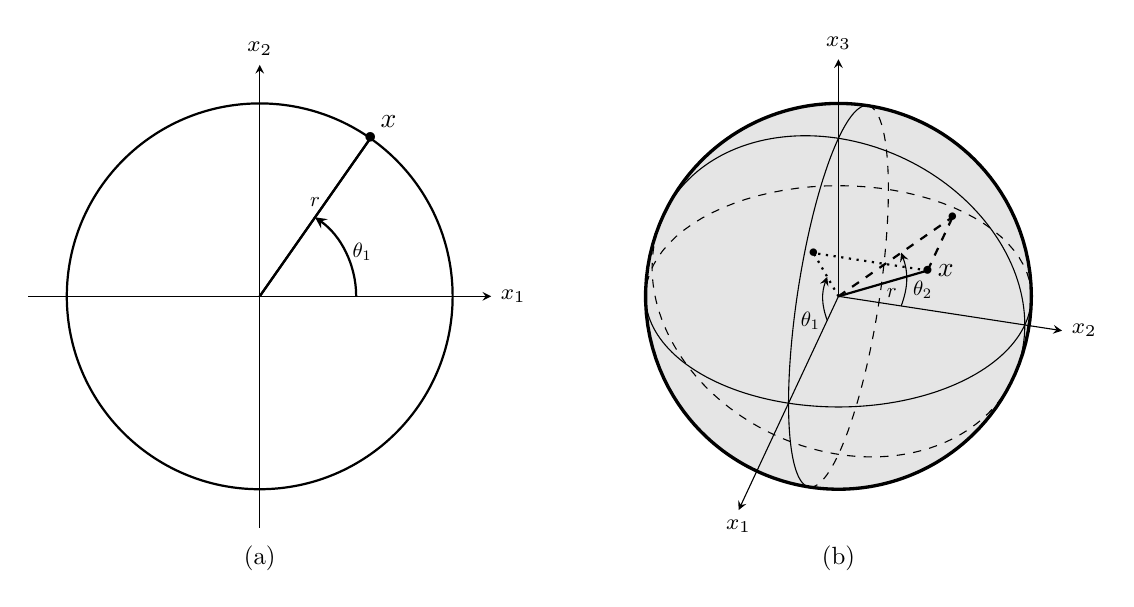
\begin{tikzpicture}[scale=.7]
\shorthandoff{>}

% CUIDADO
% Para el dibujo de la esfera, todo era hecho  en coordenadas esfericas de fisica (theta,phi)
% Para el punto x, se usan las coordenadas como en el libro, (theta_1,theta_2)
% (on dos parametrizaciones de la misma cosa...)
%
% Proyeccion para diburar un punto (x_1,x_2,x_3) teniendo en cuenta el angulo de vision
\pgfmathdeclarefunction{projx}{2}{\pgfmathparse{#1*cos(\Az)-#2*sin(\Az)}}
\pgfmathdeclarefunction{projy}{3}{\pgfmathparse{#1*sin(\Az)*sin(\El)+#2*cos(\Az)*sin(\El)+#3*cos(\El)}}


% unas definiciones para elegir el angolu de vision
\pgfmathsetmacro{\El}{35} % Elevacion
\pgfmathsetmacro{\Az}{-105}% Azimuth
%
\pgfmathsetmacro\r{3.5} % radio del circulo (d=2) y de la esfera (d=3)
%
%
% punto x para el caso d = 2
\pgfmathsetmacro\tpbi{55} % theta_1
\pgfmathsetmacro\xpbi{\r*cos(\tpbi)} % x_1
\pgfmathsetmacro\ypbi{\r*sin(\tpbi)} % x_2
%
%
% punto x para el caso d = 3
\pgfmathsetmacro\tu{60} % theta_1 punto x
\pgfmathsetmacro\td{45} %theta_2 punto x
\pgfmathsetmacro\xp{\r*cos(\tu)} % x_1 de x
\pgfmathsetmacro\yp{\r*sin(\tu)*cos(\td)} % x_2 de x
\pgfmathsetmacro\zp{\r*sin(\tu)*sin(\td)} % x_3 de x
%\pgfmathsetmacro\xp{\rp*cos(\tp)*cos(\pp)} % x_1 de x
%\pgfmathsetmacro\yp{\rp*sin(\tp)*cos(\pp)} % x_2 de x
%\pgfmathsetmacro\zp{\rp*sin(\pp)} % x_3 de x
%
%
% funcion permitiendo calcular phi(theta) dando la linea de cumbre
\pgfmathdeclarefunction{phicr}{1}{\pgfmathparse{
atan((sin(#1)*cos(\Az)+cos(#1)*sin(\Az))/(tan(\El)))
}}
%
% ====================================================================
%
% -----------------
% | Circulo d = 2 |
% -----------------
%
\begin{scope}
%
%  axes
% ------
%
\draw[>=stealth, ->] ({-1.2*\r},0)--({1.2*\r},0) node[right] {\footnotesize $x_1$};
\draw[>=stealth, ->] (0,{-1.2*\r})--(0,{1.2*\r}) node[above] {\footnotesize $x_2$};
%
%
%  Circulo
% --------
%
\draw[thick] (0,0) circle (\r);
%
%\draw (\r,0) node[below]{$r$};
%
%
%  punto x, r, theta_1
% --------------------
%
\draw[thick] (0,0) -- (\xpbi,\ypbi) node[scale=.9]{$\bullet$};
\draw[thick] (0,0) -- (\xpbi,\ypbi) node[above right]{$\boldsymbol{x}$};
\draw ({\xpbi/2},{1.05*\ypbi/2}) node[above,scale=.75]{$\boldsymbol{r}$};
\draw[->,>=stealth,thick] ({\r/2},0)  arc (0:\tpbi:{\r/2});
\draw ({\r*cos(\tpbi/2)/2},{\r*sin(\tpbi/2)/2}) node[right,scale=.75] {$\boldsymbol{\theta_1}$};
%
\node at (0,{-\r-1.25}) [scale=.9]{(a)};
\end{scope}
%
%
% ====================================================================
%
% ----------
% | Esfera |
% ----------
%
\begin{scope}[xshift=10.5cm]
%
%
%  angulo de visibilidad
% -----------------------
%
\pgfmathsetmacro\tv{-\Az}
%
%
% Axes
% -----
%
\draw[>=stealth, ->] (0,0)--({projx(\r*2,0)},{projy(\r*2,0,0)}) node[below]
{\footnotesize $x_1$};
\draw[>=stealth, ->] (0,0)--({projx(0,\r*1.2)},{projy(0,\r*1.2,0)}) node[right]
{\footnotesize $x_2$};
\draw[>=stealth, ->] (0,0)--(0,{projy(0,0,\r*1.5)}) node[above]
{\footnotesize $x_3$};
%
%
% Esfera
% ------
%
% interior de la esfera / linea de cumbre
\filldraw[very thick, domain=-\Az:-\Az+360, variable=\t, samples=180, fill opacity=.1]
plot ({projx(\r*cos(\t)*cos(phicr(\t)),\r*sin(\t)*cos(phicr(\t)))} , 
      {projy(\r*cos(\t)*cos(phicr(\t)),\r*sin(\t)*cos(phicr(\t)),\r*sin(phicr(\t)))});
%
% Ecuador (para visualisar la esfera), dado por phi = 0:
% parte visible
\draw[domain=-\Az+180:-\Az+360, variable=\t, samples=90]
plot ({projx(\r*cos(\t),\r*sin(\t))},{projy(\r*cos(\t),\r*sin(\t),0)});
%
% partie invisible
\draw[dashed, domain=-\Az:-\Az+180, variable=\t, samples=45]
plot ({projx(\r*cos(\t),\r*sin(\t))},{projy(\r*cos(\t),\r*sin(\t),0)});
%
% Linea de longitud para que se vea bien la surfaza: theta = 0 y 90
% parte visible theta = 0
\draw[domain=phicr(0):phicr(0)+180, variable=\p, samples=90]
plot ({projx(\r*cos(\p),0)},{projy(\r*cos(\p),0,\r*sin(\p))});
%
% partie escondida theta = 0
\draw[dashed, domain=phicr(0)+180:phicr(0)+360, variable=\p, samples=90]
plot ({projx(\r*cos(\p),0)},{projy(\r*cos(\p),0,\r*sin(\p))});
%
% parte visible theta = 90
\draw[domain=phicr(90):phicr(90)+180, variable=\p, samples=90]
plot ({projx(0,\r*cos(\p))},{projy(0,\r*cos(\p),\r*sin(\p))});
%
% partie escondida theta = 90
\draw[dashed, domain=phicr(90)+180:phicr(90)+360, variable=\p, samples=90]
plot ({projx(0,\r*cos(\p))},{projy(0,\r*cos(\p),\r*sin(\p))});
%
%
% Punto
% ------
%
%
% Posicion del punto x
\draw[thick] (0,0) --
({projx(\xp,\yp},{projy(\xp,\yp,\zp)})
node[scale=.75]{$\bullet$};
%
\draw[thick]
({projx(\xp,\yp},{projy(\xp,\yp,\zp)})
node[right]{$\boldsymbol{x}$};
%
%
% proyecciones para poner los angulos
% x1 = 0
%\draw[thick,dashed] ({projx(\xp,\yp},{projy(\xp,\yp,\zp})--({projx(0,\yp},{projy(0,\yp,\zp});
%\draw[thick,dashed] (0,0)--({projx(0,\yp},{projy(0,\yp,\zp});
%\draw[thick,dashed] ({projx(0,\yp},{projy(0,\yp,0})--({projx(0,\yp},{projy(0,\yp,\zp});
%
%
% notacion del radio
\pgfmathsetmacro{\propr}{.6} % distancia del radio para anotar "r"
\draw ({projx(\propr*\xp,\propr*\yp},{projy(\propr*\xp,\propr*\yp,\propr*\zp})
node[below,scale=.75] {$\boldsymbol{r}$};
%
%
% notacion del angulo theta_1
\pgfmathsetmacro{\proptu}{.45} % "radio" para dibujar el angulo
\draw[thick,dotted] ({projx(\xp,\yp},{projy(\xp,\yp,\zp})--({projx(\xp,0},{projy(\xp,0,\zp});;% proy x2=0
\draw[thick,dotted] (0,0)--({projx(\xp,0},{projy(\xp,0,\zp}) node[scale=.7]{$\bullet$};% proy x2=0
\draw[->,>=stealth]
({projx(\proptu*\xp,0)},{projy(\proptu*\xp,0,0)}) to [bend left=20]
node[pos=0,left,scale=.75] {$\boldsymbol{\theta_1}$}
({projx(\proptu*\xp,0)},{projy(\proptu*\xp,0,\proptu*\zp)});
%
%
% notacion del angulo theta_2
\pgfmathsetmacro{\propp}{.55} % "radio" para dibujar el angulo
\draw[thick,dashed] ({projx(\xp,\yp},{projy(\xp,\yp,\zp})--({projx(0,\yp},{projy(0,\yp,\zp});;% proy x1=0
\draw[thick,dashed] (0,0)--({projx(0,\yp},{projy(0,\yp,\zp}) node[scale=.7]{$\bullet$};% proy x1=0
\draw[->,>=stealth]
({projx(0,\propp*\yp)},{projy(0,\propp*\yp,0)}) to [bend right=20]
node[pos=0.3,right,scale=.75] {$\boldsymbol{\theta_2}$}
({projx(0,\propp*\yp)},{projy(0,\propp*\yp,\propp*\zp)});
%
\node at (0,{-\r-1.25}) [scale=.9]{(b)};
\end{scope}
%
\end{tikzpicture}
 \end{center}
% 
\leyenda{Coordenadas hiperesfericas para un punto dado de $\Rset^d$. (a) caso $d
  = 2$ y (b) caso $d = 3$.}
%
\label{Fig:MP:CoordenadasHiperesfericas}
\end{figure}

En  el caso  de vector  a simetr\'ia  esferica, aparece  que el  rayo $R$  y los
angulos     son     independientes      y     se     puede     calcular     cada
distribuci\'on~\cite{FanKot90, Lor54, Zoz, toto, titi}:
%
\begin{teorema}
  Sea  \  $X  \sim  \ED(0,I,d_X)$  \  y \  su  representaci\'on  en  coordenadas
  hiperesfericas \  $X_i = R \left( \prod_{k=1}^{i-1}  \sin\Theta_k \right) \cos
  \Theta_i, \quad 1 \le  i \le d$. Entonces $R$ y los $\Theta_i,  \: 1 \le i \le
  d-1$ \ son independientes y
  %
  \[
  p_R(r) = \frac{2  \pi^{\frac{d}{2}}}{\Gamma\left( \frac{d}{2} \right)} r^{d-1}
  d_X\left( r^2 \right)
  \]
  %
  \[
  p_{\Theta_i}(\theta_i)        =       \frac{\Gamma\left(       \frac{d-j+1}{2}
    \right)}{\sqrt{\pi}   \,  \Gamma\left(   \frac{d-j}{2}  \right)}   \,  \big(
  \sin\theta_i \big)^{d-i-1}  \, \un_{[0 \;  \pi)}(\theta_i), \quad 1 \le  i \le
  d-2 , \qquad p_{\Theta_{d-1}}(\theta_{d-1}) =  \frac{1}{2 \pi} \, \un_{[0 \; 2
    \pi)}(\theta_{d-1})
  \]
  %
%  y
%  %
%  \[
%  p_{\Theta_{d-1}}(\theta_{d-1})   =   \frac{1}{2   \pi}   \,   \un_{[0   \;   2
%    \pi)}(\theta_{d-1})
%  \]
\end{teorema}
%
\begin{proof}
  Sea      la       transformaci\'on      $g:      (x_1,\ldots,x_d)      \mapsto
  (r,\theta_1,\ldots,\theta_{d-1})$. La jacobiana de $g^{-1}$ tiene la forma
  %
  \[
  \Jac_{g^{-1}} = \begin{bmatrix}
  %
    \frac{\partial x_1}{\partial r} & \frac{\partial x_1}{\partial \theta_1} & 0 & \cdots & 0\\
  %
    \vdots & \vdots & \ddots & \ddots & \vdots\\
  %
    \vdots & \vdots &  & \ddots  & 0\\
  %
    \frac{\partial x_{d-1}}{\partial r} & \frac{\partial x_{d-1}}{\partial
    \theta_1} & \cdots & & \frac{\partial x_{d-1}}{\partial \theta_{d-1}}\\
  %
    \frac{\partial x_d}{\partial  r} & \frac{\partial  x_d}{\partial \theta_1} &
    \cdots & \cdots & \frac{\partial x_d}{\partial \theta_{d-1}}
  %
  \end{bmatrix}
  \]
  %
  Desarrolando   el   determinante  por   la   \'ultima   columna  por   ejemplo
  (ver~\cite{Bha97, HorJoh13}), y as\'i por inducci\'on se obtiene
  %
  \[
  \left|   \Jac_{g^{-1}}  \right|  =   r^{d-1}  \prod_{j=1}^{d-2}   \left(  \sin
    \theta_i\right)^{d-j-1}
  \]
  %
  Entonces,  por  transformaci\'on  (ver  secci\'on~\ref{Sec:MP:Transformacion})
  tenemos
  %
  \[
  f_{R,\Theta_1,\ldots,\Theta_{d-1}}(r,\theta_1,\ldots,\theta_{d-1}) = d_X\left(
    r^2    \right)     r^{d-1}    \prod_{j=1}^{d-2}    \left(     \left(    \sin
      \theta_i\right)^{d-j-1} \un_{[0 \; \pi)}(\theta_i) \right) \, \un_{[0 \; 2
    \pi)}(\theta_{d-1})
  \]
  %
  Claramente  se  factoriza  probando  la  independencia  y  la  forma  de  cada
  distribuci\'on   marginal.    El   factor   viene    de   la   normalizaci\'on
  (ver~\cite[Ec.~8.380-2]{GraRyz15}   para  los   angulos,   lo  que   determina
  necesariamente el del rayo).
\end{proof}
%
Obviamente,   se   recupera   la   ley   de   \   $R   \egald   \|X\|$   \   que
encontramos.  Ad\'emas, estas coordenadas  hiperesfericas, a  $r=1$, parametriza
$\Sset_d$  y permite  por ejemplo  de probar  la independencia  entre  $\|X\|$ y
$\frac{X}{\|X\|}$ (y entonces la  escritura en mezcla), de calcular directamente
\ $\Phi_U(\omega)$ \ para \ $U  \sim \U(\Sset_d)$, o de vincular las generadoras
caracter\'istica y de densidad entre otros.

En la familia  eliptica, hay una subfamilia particular  que queda invariante por
marginalizaci\'on, y extensi\'on, como la gausiana por ejemplo:
%
\begin{definicion}[Consistencia~\cite{Yao73, Kan94}]
%
  Sea \  $X = \begin{bmatrix} X_1 &  \cdots & X_d \end{bmatrix}$  \ a simetr\'ia
  eliptica  de  generadora  de  densidad  $d_X$.   Este  vector  es  dicho  {\em
    consistente}   si  la   generadora  de   densidad  \   $d_{X'}$  \   de  $X'
  = \begin{bmatrix} X_1 & \cdots &  X_{d'} \end{bmatrix}$ \ tiene la misma forma
  que \ $d_X$  \ donde el par\'ametro  dimensional \ $d$ \ es  reemplazado por \
  $d'$.  En  otros termoinos tenemos  invarianza por marginalizaci\'on si  $d' <
  d$, pero se puede ver $X$ como marginal de un vector m\'as grande con la misma
  generadora de probabilidad re-emplazando $d$ por $d'$.

  Se proba  que, equivalentemente, la generadora caracteristica  \ $\varphi_X$ \
  no  es  relacionada a  \  $d$  (ver~\cite{Kan94,  FanKot90} para  la  prueba).
  Entonces, $\varphi_X$  va a ser  una generadora caracter\'istica de  un vector
  aleatorio   de  cualquier   dimensi\'on  \   $d  \in   \Nset^*$,  o,   con  la
  caracterisaci\'on por functiones definida positivas (ver teorema de Bocher), \
  $\varphi_X   \in  \PDSI$  (ver   notaciones,  y   las  a   continuaci\'on  del
  teorema~\ref{Teo:MP:GeneradorasCaracteristicas}).
%$\omega \mapsto \varphi_X\left(
%    \| \omega  \|^2 \right) \, \in  \, \PD$ \ conjuntos  de funci\'on hermiticas
%  definidas    positivas,     unidad    al    origen     (ver    notaciones    o
%  secci\'on~\ref{Ssec:MP:Generadoras}).
\end{definicion}


Si \  $X$ \  a simetr\'a  esferica (y por  transformaci\'on af\'in  a simetr\'ia
eliptica)  se escribe  siempre  como mezcla  de  escala de  base uniforme,  esta
escritura estocastica no es \'unica. Por  ejemplo, si consideramos $X = A \, G$,
con \
%$m \in \Rset^d$, , $\Sigma \in P_d^+(\Rset)$, 
$A$ \ variable  aleatoria positiva \ y \ $G \sim  \N(0,I)$ independiente de $G$,
queda claro que \ $X$ \  es a simetr\'ia esferica. Estos vectores, llamados {\em
  mezcla  de escala  de  base gausiana},  o  simplemente {\em  mezcla de  escala
  gausiana}  (GSM para  Gaussian scale  mixture en  ingl\'es)  fueron estudiados
intensivamente de manera formal~\cite{Kan94,  Yao73, Ver64, Pic70, Kel71, Kin72,
  KeiSte74, Tei60, AndMal74}.  Ecuentra aplicaciones en varias area, modelizando
la  textura  de imagenes  o  data  de radar  (e.g.   suma  aleatoria de  vecores
gausianos)~\cite{PorStr03,   BomBea08,  Sel08,  ShiSel07,   ZozVig10,  TisNic04,
  TodTab07}.

Una  pregunta natural  es  de saber  si  se puede  escribir  cualquier vector  a
simetr\'a  esferica como mezcla  de escala  de base  gausiana.  La  respuesta es
negativa. Por ejemplo,  del dominio de definici\'on de  la variable, queda claro
que un  vector uniforme sobre la  esfera no puede  ser mezcla de escala  de base
gausiana (ver  un otro contra-ejemplo en~\cite{Pic70}).  Escribir  un vecor como
tal mezcla  resuelte posible  solamente bajo restricciones.  M\'as precisamente,
una condici\'on necesaria  y sufiente est que la  variable debe ser consistente,
como    lo    prob\'o    tambi\'en    Sch{\oe}nberg~\cite[Teo.~2]{Sch38}    (ver
tambi\'en~\cite[Teo.~2]{SteVan05},            \cite[Lem.~2.2]{Yao73}           o
\cite[Teo.~1]{Kan94}).
%
\begin{teorema}[Sch{\oe}berg'38 -- a partir de la generadora caracter\'istica]
\label{Teo:MP:SchoenbergCaracteristica}
%
  Sea \ $X \sim  \ED\left( m , \Sigma , \varphi_X \right)$.  Entonces $X$ es una
  mezcla de  gausiana si y  solamente si $X$  es consistente, es decir
  % lo que se escribe tambi\'en, con $Y = \sigma^{-\frac12} (X-m)$,
  %
  \[
  X \,  \egald \,  A \, \Sigma^{\frac12}  \, G  + m \quad  \Leftrightarrow \quad
  \varphi_X \in \PDSI
  \]
  %
  con \ $A > 0$ \ independiente de \ $G \sim \N(0,I)$.
\end{teorema}
%
\begin{proof}
  La directa es inmediata de la formula de esperanza total
  %
  \[
  \varphi_X(w)  =  \Esp\big[ \,  \Esp\left[  \varphi_G\left( A w \right)  \left.  \right|
      A\right] \, \big]
  \]
  %
  conjuntamente a \ $\varphi_G: w \mapsto e^{-\frac{w}{2}} \: \in \PDSI$.

  La reciproca es  m\'as dificil a probar. Para los  detalles, dejamos el lector
  a~\cite{Sch38}. Los  elementos de prueba  son los siguientes. De  la escritura
  como mezcla de escala uniforme tenemos entonces para cualquier \ $d$
  %
  \[
  \varphi_X\left(  w^2  \right)   =  2^{\frac{d}{2}-1}  \Gamma\left(  \frac{d}{2}
  \right) \int_{\Rset_+} \left(  w r \right)^{1-\frac{d}{2}} J_{\frac{d}{2}-1}(w
  r) \, dP_{R_d}(r)
  \]
  %
  con \  $R_d$ \ la  variable generadora de  base uniforme correspondiente  a la
  dimension   $d$   (ver   prueba  del   teorema~\ref{Teo:MP:MezclaUniforme}   y
  ejemplo~\ref{Ej:MP:GeneCaracUniformeEsfera}).  Por   cambio  de  variables  se
  escribe tambi\'en
  %
  \[
  \varphi_X\left(  w^2 \right)  = \int_{\Rset_+}  2^{\frac{d}{2}-1} \Gamma\left(
    \frac{d}{2}   \right)   \left(    w   r   \sqrt{d}   \right)^{1-\frac{d}{2}}
  J_{\frac{d}{2}-1}\left(  w r  \sqrt{d}  \right) \,  dP_{R_d}\left( r  \sqrt{d}
  \right)
  \]
  %
  Eso siendo  valid en cualquier orden,  se nota $P_R$ el  l\'imite de $P_{R_d}$
  cuando $d$ tiende al infinito.  Luego,  el desarollo de Taylor de la funci\'on
  de Bessel  y de  la f\'ormula de  Stirling~\cite[Ec.~8.402~y~8.327]{GraRyz} se
  proba que
  %
  \[
  \lim_{d \to +\infty} 2^{\frac{d}{2}-1} \Gamma\left( \frac{d}{2} \right) \left(
    w  r \sqrt{d} \right)^{1-\frac{d}{2}}  J_{\frac{d}{2}-1}\left( w  r \sqrt{d}
  \right) \: = \: e^{-\frac{w^2 r^2}{2}}
  \]
  %
  Todo el  juego consiste a probar  que la convergencia es  uniforme, para poder
  intercambiar   l\'imite   e    integral.    Dio   una   prueba   Sch{\oe}nberg
  en~\cite{Sch38},  y  luego  propuso  un  ``m\'as moderna''  Steerneman  y  van
  Perlo-ten-Kleij  en~\cite{SteVan05}.  Basicamente  se reconoce  en  $w \mapsto
  2^{\frac{d}{2}-1}   \Gamma\left(  \frac{d}{2}   \right)   \left(  w   \sqrt{d}
  \right)^{1-\frac{d}{2}}   J_{\frac{d}{2}-1}\left(  w   \sqrt{d}   \right)$  la
  funci\'on  caracter\'istica  de  $q_d(x)  \propto  \left(  1  -  \frac{x^2}{d}
  \right)_+^{\frac{d-3}{2}}$  \  que  tiende  a  la gausiana  (ver  por  ejemplo
  secci\'on~\ref{Sssec:MP:StudentR}).   Se usa el  lema de  Scheff\'e o  de Riez
  (ver~\cite{Rie28,  Sch47, Nov72,  Kus10} o  \cite{AthLah06,  Bog07:v1, Bil12})
  para probar la convergencia de la integral.
% (es similar al uso del teorema de convergencia dominada).
\end{proof}
%
\noindent Se encuentra una prueba alternativa tambi\'en en~\cite{FanKot90, Kin72}.

Este  teorema pone  en  juega la  condici\'on  necesaria y  suficiente sobre  la
funci\'on caracter\'istica para  tener una mezcla de escala  gausiana, as\'i que
no es necesario que \ $X$ \ admita una densidad de probabilidad. sin embargo, al
imagen de la  consistencia que se exprime tambi\'en a  trav\'es de la generadora
de  densidad,  el  teorema  de  Sch{\oe}nber tiene  una  versi\'on  usando  esta
generadora.   Por  eso,  introducimos  el conjunto  de  funciones  complatemente
monotonas   sobre  $\Rset_+$   hasta   un  cierto   orden,   y  para   cualquier
orden~\footnote{Una funci\'on  \ $f: I \subset  \Rset \mapsto \Rset$  \ es dicha
  {\em absolutamente monotona} si es continua, diferenciable a todos los ordenes
  en el interior of $I$, y todas sus derivadas son positivas, $ \forall \: k \in
  \Nset, \quad f^{(k)} \ge 0$.  $f$ \ es dicha {\em completamente monotona} si \
  $f(-x)$ \ es absolutamente monotona~\cite{Ber29}.} (ver notaciones):
%
\[
\CM_n = \left\{ f \in C^{n-1}(\Rset_+) \tq \forall \, k = 0 , \ldots , n-1, \:\:
  (-1)^k  f^{(k)}  \ge 0  \:  \et \:(-1)^k  f^{(k)}  \:  \mbox{ es  decreciente}
\right\}
\]
%
y
%
\[
\CM = \bigcap_{n=0}^{+\infty} \CM_n =  \left\{ f \in
  C^{\infty}(\Rset_+)  \tq \forall \,  k \in  \Nset, \:\:  (-1)^k f^{(k)}  \ge 0
\right\}
\]
%
\begin{teorema}[Sch{\oe}berg'38 -- a partir de la generadora de densidad]
\label{Teo:MP:SchoenbergDensidad}
%
  Sea \ $X \sim \ED\left( m , \Sigma , d_X \right)$.  Entonces $X$ es una mezcla
  de  gausiana  si  y  solamente   si  $d_X$  es  completamente  monotona  sobre
  $\Rset_+$
  % lo que se escribe tambi\'en, con $Y = \sigma^{-\frac12} (X-m)$,
  %
  \[
  X \, \egald \, A \, \Sigma^{\frac12}  \, G + m \quad \Leftrightarrow \quad d_X
  \in \CM
  \]
  %
  con \ $A > 0$ \ independiente de \ $G \sim \N(0,I)$.
\end{teorema}
%
\begin{proof}
  La prueba se apoya sobre el teorema de Haussdorf-Bernstein-Widder que proba la
  equivalencia entre la  clase de funciones completamente monotonas  y la de las
  funciones   \   $f$   \   que   se   escriben   como   una   transformada   de
  Laplace-Stieltjes~\footnote{Por     definici\'on,    la     transformada    de
    Laplace-Stieltjes de una medida \ $\mu$  \ definida sobre $\Rset_+$ \ es una
    funci\'on   de  un   n\'umero  complejo   \  $\displaystyle   \LS[\mu](s)  =
    \int_{\Rset_+} e^{-s t}  \, d\mu(t)$. Se proba que un  real \ $x_0$, llamado
    abscisa de convergencia tal que  la convergencia es uniform en el semi-plano
    \ $\real{s} > x_0$, y a  continuaci\'on tal que \ $\displaystyle \LS[\mu]$ \
    es analitica en este semi-plano.   Si \ $\displaystyle \mu = \sum_i \alpha_i
    \delta_{t_i}$  \  es  una   medida  discreta  se  obtiene  \  $\displaystyle
    \LS[\mu](s)  =  \sum_i  \alpha_i  e^{-s  t_i}$  \  conocido  como  seria  de
    Dirichelt,  y  si  \ $\mu$  \  admite  una  densidad \  $g$,  $\displaystyle
    \LS[\mu](s) \equiv  \L[g](s) = \int_{\Rset_+} e^{-s  t} \, g(t) \,  dt$ \ es
    dicha transformada de Laplace ordinaria de  \ $g$.  Para $s = \imath \omega$
    \ con  $\omega \in  \Rset$, las transformaciones  de Laplace-Stieltjes  y de
    Laplace coinciden con las transformaciones $\FS$ de Fourier-Stieltjes y $\F$
    de           Fourier            ordinaria           (ver           tambi\'en
    secci\'on~\ref{Ssec:MP:FuncionCaracterisica} para esta transformaci\'on). Al
    imagen  de   la  transformada  de  Fourier  inversa   que  vimos  brevemente
    secci\'on~\ref{Ssec:MP:FuncionCaracteristica},    existen    f\'ormulas   de
    inversi\'on, denotadas \  $\LS^{-1}$ \ y \ $\L^{-1}$  \ respectivamente.  Se
    referir\'a     por    ejemplo     a~\cite{Wid46}     para    tener     m\'as
    detalles. \label{Foot:MP:LaplaceStieltjes}} (en el eje real)
  %
  \[
  f(t) = \int_{\Rset_+} e^{-t u} d\mu(u)
  \]
  %
  donde  $\mu$  es  una  medida finita  (ver~\cite[Teo.~3]{Sch38},  \cite{Ber29,
    Haus21:I, Haus21:II,  Wid32}, \cite[\S~12]{Wid46}, \cite[\S~XIII.4]{Fel71}).
  %
  % Feller v2, p.  439; Widder p. 160; Schoenberg th. 3  y sec. 4 (Hausdorff'21,
  % Bernstein'29, Carlson'21),
  % 
  Con el  cambio de variables  $u = \frac{1}{2  a^2}$ \ y  \ $\mu\big( (0  \; u)
  \big) =  (2 u)^{\frac{d}{2}} P_A\left( \left( \frac{1}{\sqrt{2  u}} \; +\infty
    \right) \right)$,  se aplica entonces este teorema  a (formula de probabilidad
  total)
  %
  \[
  d_X(r)  =  (2 \pi)^{-\frac{d}{2}} \int_{\Rset_+} a^{-d} e^{-\frac{r}{2 a^2}} dP_A(a) 
  \]

  Basicamente la  directa viene  de esta  formula de probabilidad  total y  de \
  $\displaystyle     \frac{d^k    e^{-\frac{r}{2    a^2}}}{dr^k}     =    (-1)^k
  \frac{e^{-\frac{r}{2 a^2}}}{2^k  a^{2 k}}$ \  (se usa para  poder intercambiar
  derivada    e     integral    el    teorema     de    convergencia    dominada
  sec.~\ref{Ssec:MP:VAPreliminaria}).

  De  nuevo,   la  reciproca   es  m\'as  dificil   a  probar  y   es  detallada
  en~\cite[\S~12]{Wid46} por ejemplo.  Basicamente, se  muestra que si \ $d_X$ \
  es  completamente  monotona,  se  puede  escribir \  $\displaystyle  d_X(n)  =
  \int_{\Rset_+}  v^n  d\mu(v)  =  \int_{\Rset_+}  e^{-n  u}  d\mu\left(  e^{-u}
  \right)$, momento de  orden \ $n$ con respecto a una  medida de probabilidad \
  $\mu$~\cite{Hau21:I, Hau21:II},  visto como transformada  de Laplace-Stieltjes
  en \ $t  = n$.  Se define la funci\'on \  $\displaystyle f(r) = \int_{\Rset_+}
  e^{- r  u} d\mu\left( e^{-u}  \right)$ \  que coincide con  \ $d_X$ \  sobre \
  $\Nset$.   Se  proba   finalmente  que  \  $d_X(r)  -   f(r)$  \  se  extiende
  analiticamente  en el  semi  plano  complejo \  $\real{s}  \ge 0$  \  y de  la
  analiticidad  que  \ $d_X$  \  y  \ $f$  \  coinciden  entonces  en todo  este
  plano~\cite{Car21, CarKro05}.
\end{proof}

Se  notar\'a  que  la consistencia  se  manifesta  tambi\'en  a trav\'es  de  la
generadora de la mezcla gausiana:
%
\begin{lema}\label{Lem:MP:AIndependienteD}
  Sea  \ $\varphi_X  \in  \PDSI$ (o  $d_X  \in \CM$).  Entonces, para  cualquier
  dimension \ $d$ \ y  $X \sim \ED(m,\Sigma,\varphi_X)$ \ $d$-dimensional, en la
  escritura  \ $X  \egald  A \,  \Sigma^{\frac12} G  +  m$ \  con  \ $A  > 0$  \
  independiente de \ $G  \sim \N(0,I)$ la ley de $A$ no  depende de la dimension
  $d$.
\end{lema}
%
\begin{proof}
  La  prueba  es  inmediata del  hecho  de  que  para  cualquier matriz  $M  \in
  \M_{d,n}(\Rset)$ de rango lleno con $d  \le n$, \ $X \egald A \Sigma^{\frac12}
  G $ \ con  \ $G \sim \N(0,I)$ \ $n$-dimensional, tenemos $X' =  M X \egald A M
  \Sigma^{\frac12} G \egald A \left( M  \Sigma M^t \right)^{\frac12} G'$ \ con \
  $G'         \sim        \N(0,I)$         \         $d$-dimensional        (ver
  teorema~\ref{Teo:MP:StabilidadGaussiana}). Una mezcla de gausiana queda mezcla
  de proyecci\'on,  con la misma  generadora $A$, y  al rev\'es puede  ser vista
  como proyecci\'on de una mezcla de  dimension m\'as grande (no va a cambiar la
  generadora)~\footnote{Cuidense  de que  no anda  si  salimos a  partir de  una
    mezcla  de base  uniforme: como  lo  vamos a  ver, las  proyecciones no  son
    uniforme m\'as si $d  < n$, lo que se intuite por  razones de dominio imagen
    (bolas por proyecci\'on de la esfera).}.
\end{proof}

Si  en  la  escritura  como  mezcla  de  escala  de  base  uniforme  se  escribe
sencillamente  la  ley  del rayo  \  $R$,  se  puede tambi\'en  caracterizar  la
generadora en  el caso de  mezcla de base  gausiana. Viene de la  escritura como
mezcla,       donde       se       reconoce      une       transformada       de
Laplace-Stieltjes~\footref{Foot:MP:LaplaceStieltjes}.

\begin{lema}\label{Lem:MP:PaLaplaceInversa}
  Sea \ $X \sim \ED(m,\Sigma,\varphi_X)$ \  mezcla de escala gausiana, con \ $A$
  la  variable aleatoria  generadora.  $\varphi_X$ \  admite una  continuaci\'on
  anal\'itica \ $s \mapsto \varphi_X(s)$ \ en el semi-plano complejo \ $\real{s}
  > 0$.  Notando \ $\LS$ \ la transformada de Laplace-Stieltjes y \ $\LS^{-1}$ \
  la transformada inversa  (ver nota de pie~\footref{Foot:MP:LaplaceStieltjes}),
  la funci\'on de repartici\'on de \ $A$ \ es dada por
  %
  \[
  F_A(a) = \LS^{-1}[\varphi_X] \left( \left( 0 \; \frac{a^2}{2} \right) \right)
  \]
  %
  Si la medida \ $P_A$ \ admite una densidad \ $p_A$, se obtiene inmediatamente
  %
  \[
  p_A(a) = a \, \L^{-1}[\varphi_X] \left(\frac{a^2}{2} \right)
  \]

  Similarmente, si \ $X$ \ admite una  generadora de densidad \ $d_X$, \ $d_X$ \
  se extiende tambi\'en anal\'iticamente en el semi-plano complejo \ $\real{s} >
  0$ \ y se obtiene
  %
  \[
  \int_0^a u^{-d} dP_A(u) = (2 \pi)^{\frac{d}{2}} \, \LS^{-1}[d_X] \left( \left(
      \frac{1}{2 a^2} \; +\infty \right) \right) \qquad \mbox{y} \qquad f_A(a) =
  (2 \pi)^{\frac{d}{2}} \, a^{d-3} \, \L^{-1}[d_X]\left( \frac{1}{2 a^2} \right)
  \]
  %
  respectivamente.
\end{lema}
%
\begin{proof}
  Para \ $U$ \ uniforme sobre la  esfera, del desarollo en serie de la funci\'on
  de  Bessed   \cite[Ec.~8.402]{GraRyz15},  es  claro  que   \  $\varphi_U(w)  =
  2^{\frac{d}{2}-1}  \Gamma\left(   \frac{d}{2}  \right)  \,  w^{-\frac{d-2}{4}}
  J_{\frac{d}{2}-1}(\sqrt{w})$  \  admite  una  continuaci\'on analitica  en  en
  semi-plano  complejo $\real{s}  >  0$.   De la  mezcla  uniforme, tambi\'en  \
  $\varphi_X(w)  =   \int_{\Rset_+}  \varphi_X(r  w)  \,   dP_R(r)$  admite  una
  continuaci\'on analitica en  en semi-plano complejo $\real{s} >  0$. Luego, de
  la escritura de mezcla gausiana tenemos
  %
  \[
  \varphi_X(w) = \int_{\Rset_+} e^{-\frac{w a^2}{2}} \, dP_A(a) = \int_{\Rset_+}
  e^{- w t} \, dP_A(\sqrt{2 t})
  \]
  %
  por cambio de variables donde se reconoce la transformada de Laplace-Stieltjes
  \  $\L$ \  de  la medida  \  $\mu$ \  (definida sobre  $\Rset_+$)  dada por  \
  $\mu\big( (0 \; t) \big) = P_A\left(  \left( 0 \; \sqrt{2 t} \right) \right) =
  F_A(\sqrt{2  t})$.  La  funci\'on  de repartici\'on  en  \ $\sqrt{2  t}$ \  es
  entonces dada por la transformada  inversa de Laplace-Stieljes de \ $s \mapsto
  \varphi_X(s)$, lo  que ciertra la prueba  para \ $F_A$.   Ahora, para escribir
  $p_A$ \ se puede diferenciar $F_A$ obtenido, o simplemente escribir $dP_A(a) =
  p_A(a) \, da$, \ie \ $dP_A(\sqrt{2 t}) = \frac{p_A(\sqrt{2 t})}{\sqrt{2 t}} \,
  dt$ \ y reconocer en \  $\varphi(s)$ \ la transformada ordinaria de Laplace de
  $t \mapsto \frac{p_A(\sqrt{2 t})}{\sqrt{2 t}}$.

  La prueba que \ $d_X$ \  se extiende analiticamente en el semi-plano $\real{s}
  >0 $ es dada en~\cite[Cap.~IV, Teo.~3a]{Wid46}~\footnote{Se proba de hecho que
    una  funci\'on absolutamente  monotona  sobre  $\Rset_-$, como  lo  es \  $r
    \mapsto d_X(-r)$,  se extiende analiticamente  en el semi-plano  $\real{s} <
    0$.}. Basicamente, siendo  \ $d_X$ \ $C^\infty$, se  escribe su desarollo de
  Taylor al torno de un $r_0 > 0$ y  se proba que sobre $r \in (0 \; r_0)$, esta
  serie de terminos todos positivos converge uniformamente. Por consecuencia, se
  tiene la convergencia uniforme tambi\'en para \  $r = s$ \ en la bola compleja
  \ $|s-r_0|  < r_0$. Se cierra  la prueba de  la validez para cualquier  $r_0 >
  0$. A continuaci\'on, la forma de \ $P_A$ \  y \ $p_A$ \ a partir de \ $d_X$ \
  viene de los mismos pasos, saliendo de
  %
  \[
  d_X(r) =  \int_{\Rset_+} (2 \pi)^{-\frac{d}{2}} \,  a^{-d} e^{-\frac{r}{2}} \,
  dP_A(a) = (2 \pi)^{\frac{d}{2}}  \, \int_{\Rset_+} (2 t)^{\frac{d}{2}} \, e^{-
    w t} \, dP_A\left( (2 t)^{-\frac12} \right)
  \]
  %
  y introduciendo la medida \ $\mu_A$ \ definida por \ $\displaystyle \mu_A(B) =
  \int_B (2  t)^{\frac{d}{2}} \, dP_A\left(  (2 t)^{-\frac12} \right)$ \  por un
  lado, y escribiendo \ $dP_A(a) = p_A(a) da$ \ por el otro lado.
\end{proof}

Cuando se puede extender \ $\varphi_X$ \  o \ $d_X$ \ al eje complejo imaginario
puro, $w  = \imath \, \omega$ \  o \ $r =  \imath \, \omega$ \  se remplazan las
transformadas de Laplace-Stieltjes y Laplace ordinarias (y sus inversas) por las
de  Fourier-Stieltjes   \  $\FS$\   y  Fourier  ordinaria   \  $\F$  \   (y  sus
inversas)~\footnote{Se   puede  tambi\'en  pensar   a  la   transformaci\'on  de
  Mellin-Stieltjes   y  la   de  Mellin   ordinario  dada   respectivamente  por
  $\displaystyle  \MS[\mu](s) =  \int_{\Rset_+} t^s  \, d\mu(t)$  \quad  y \quad
  $\displaystyle  \M[g](s) = \int_{\Rset_+}  t^{s-1} \,  g(t) \,  dt$, definidas
  sobre una  banda del  plano complejo del  tipo \  $\real{s} \in (x_m  \; x_M)$
  (abscisas de convergencia), \  y usar sus propiedades remarcables~\cite{Zol57,
    Pou99, Pou10,  Wid46, ParKam01}.   En el caso  con densidad por  ejemplo, se
  reconoce en \  $g_X(r) = r^{d-1} d_X\left( r^2 \right)$ \  (ley del rayo, bajo
  un factor) lo  que se llama convoluci\'on af\'in, entre \  $g_G(r)$ \ (ley del
  rayo  de  la gausiana)  \  y  la medida  de  \  $A$,  $\displaystyle g_X(r)  =
  \int_{\Rset_+} \frac{1}{a} g_G\left( \frac{r}{a} \right) \, p_A(a) \, da$.  Al
  imagen de las  propiedades de la transformada de  Laplace, la transformaci\'on
  de Mellin de  una convoluci\'on af\'in es el  producto de las transformaciones
  de Mellin, y por un lado \ $\M[t^\alpha g(t)](s) = \M[g](s+\alpha)$ \ y por el
  otro lado  \ $\M[g(r^\alpha)](s) = |\alpha|^{-1}  \M[g](s/\alpha)$.  As\'i, se
  obtiene  sencillamente,  de  \  $\M[d_G](s)  =  2^s  \Gamma(s)$~\cite[Cap.~12,
  Tabla~12.1]{Pou10}   o~\cite[Cap.~18,  Tabla~18.1]{Pou99}   \   $\M[p_A](s)  =
  \frac{\pi^{\frac{d}{2}}              \M[d_X]\left(             \frac{s+d-1}{2}
    \right)}{2^{\frac{s-1}{2}} \Gamma\left( \frac{s+d-1}{2} \right)}$.
  % \ para \ $\real(s) > 1-d$.
  Similarmente,  se  muestra  en  el  caso  con densidad  que  \  $\M[p_A](s)  =
  \frac{\M[\varphi_X]\left(       \frac{1-s}{2}       \right)}{2^{\frac{1-s}{2}}
    \Gamma\left( \frac{1-s}{2} \right)}$,
  % \ para \ $\real{s} < 1$,
  \   y   \   obviamente   \  $\M[\varphi_X]   =   \frac{\pi^{\frac{d}{2}}   4^s
    \Gamma(s)}{\Gamma\left( \frac{d}{2} - s \right)} \M[d_X]\left( \frac{d}{2} -
    s  \right)$ \  (lo que  se obtiene  tambien a  partir de  la  relaci\'on via
  transformada de  Hankel entre esta generadoras). Se  puede referirse tambi\'en
  a~\cite[\S~3.2.1]{Zoz12}).  }
%
\cite{Zol57, Pou99, Pou10, Wid46, ParKam01}.

\

Varios  vectores aleatorios que  hemos visto  caen en  la familia  eliptica.  No
admiten todas  una densidad con respecto a  la medida de Lebesgue,  como lo hemos
visto con la ley uniforme sobre la esfera (admite una con respecto a la medida de
Haar), tampoco no  son todas consistentes (y entonces no  se escriben todas como
mezcla de escala de base gausiana).
%
\begin{ejemplo}[Distribuci\'on gausiana]
%
  Sea \ $X \sim \N(m,\Sigma)$.  Entonces, \ $X \sim \ED(m,\Sigma,\varphi_X)$ \ o
  equivalentemente \ $X \sim \ED(m,\Sigma,d_X)$ con
  %
  \[
  \varphi_X(u) =  e^{-\frac{u}{2}} \qquad \mbox{y}  \qquad , \qquad d_X(r)  = (2
  \pi)^{-\frac{d}{2}} e^{- \frac{r}{2}}
  \]
  
  Eso da la ley del rayo
  %
  \[
  p_R(r)  =  \frac{1}{2^{\frac{d}{2}-1}  \Gamma\left(  \frac{d}{2}  \right)}  \:
  r^{d-1} e^{- \frac{r^2}{2}}
  \]
  %
  Aparece   que  \   $R^2  \sim   \G\left(  \frac{d}{2}   ,   \frac12\right)$  \
  distribuci\'on Gamma.
  
  Adem\'as,   la  generadora   caracter\'istica  siendo   independiente   de  la
  dimensi\'on \  $d$, \  $\Phi_X \in \PD$,  o equivalentemente la  generadora de
  densidad  \ $d_X$ \  teniendo la  forma que  damos para  cualquier dimensi\'on
  (cambiar  de  dimensi\'on  es  equivalente  a cambiar  $d$),  la  gausiana  es
  consistente;  Las  marginales  de  una  gausiana son  gausianas,  y  cualquier
  gausiana puede ser  vista como marginale de gausiana  de cualquier dimensi\'on
  m\'as grande.

  Obviamente, se  escribe como  mezcla de  escala de gausiana  con \  $A =  1$ \
  variable cierta.
\end{ejemplo}

\begin{ejemplo}[Distribuci\'on Student-$t$]
%
  Sea \ $X \sim \T_\nu(m,\Sigma)$.  Entonces, \ $X \sim \ED(m,\Sigma,\varphi_X)$
  \ o equivalentemente \ $X \sim \ED(m,\Sigma,d_X)$ con
  %
  \[
  \varphi_X(u)   =  \frac{\nu^{\frac{\nu}{4}}}{2^{\frac{\nu}{2}-1}  \Gamma\left(
      \frac{\nu}{2}   \right)}   \,  u^{\frac{\nu}{4}}   K_{\frac{\nu}{2}}\left(
    \sqrt{\nu \,  u} \right) \qquad \mbox{y} \qquad  d_X(r) = \frac{\Gamma\left(
      \frac{d+\nu}{2}     \right)}{(\pi     \nu)^{\frac{d}{2}}     \Gamma\left(
      \frac{\nu}{2}    \right)}   \left(    1    +   \frac{r}{\nu}    \right)^{-
    \frac{d+\nu}{2}}
  \]

  Se obtiene de \ $d_X$ \ la ley de rayo
  %
  \[
  p_R(r)  =  \frac{2}{\nu^{\frac{d}{2}}   B\left(  \frac{\nu}{2}  ,  \frac{d}{2}
    \right)} \:
  % \frac{2    \,   \Gamma\left(    \frac{d+\nu}{2}   \right)}{\nu^{\frac{d}{2}}
  %   \Gamma\left( \frac{\nu}{2} \right) \Gamma\left( \frac{d}{2} \right)} \,
  \frac{r^{d-1}}{\left( 1 + \frac{r^2}{\nu} \right)^{\frac{d+\nu}{2}}}
  \]
  %
  Con \ $F = \frac{R^2}{d}$ \ se obtiene por transformaci\'on
  %
  \[
  p_F(f)   \propto   \frac{f^{\frac{d}{2}-1}}{\left(   1   +   \frac{d}{\nu}   f
    \right)^{\frac{d+\nu}{2}}}
  \]
  %
  conocido como ley de Fisher-Snedecor (o $F$), de grados de libertad $(d,\nu)$,
  o tipo Pearson VI, o  beta de secunda especie~\cite{JohKot95:v2, Muk00, Bre88,
    IbaPer12} (ratio de Gamma independientes).

  La Student-$t$ es tambi\'en consistence de la independencia de \ $\varphi_X$ \
  con la dimensi\'on \ $d$, \  $\Phi_X \in \PD$, o equivalentemente del hecho de
  que  la generadora de  densidad \  $d_X$ \  teniendo la  forma que  damos para
  cualquier dimensi\'on  (cambiar de dimensi\'on es equivalente  a cambiar $d$);
  Las  marginales de  una Student-$t$  con \  $\nu$ \  grados de  libertad queda
  Student-$t$ con  $\nu$ grados  de libertad y  cualquier Student-$t$  con $\nu$
  grados de  libertad pued ser vista  como marginal de un  Student-$t$ con $\nu$
  grados de libertad de cualquier dimensi\'on m\'as grande.

  V\'imos           en           la           secci\'on~\ref{Sssec:MP:StudentT},
  lema~\ref{Lem:MP:MezclaGaussianaEscalaStudentT},    que    se   escribe    una
  Student-$t$   como   mezcla   de   escala   Gausiana   donde   \   $A   \egald
  \frac{1}{\sqrt{V}},  \: V \sim  \G\left( \frac{\nu}{2}  \, ,  \, \frac{\nu}{2}
  \right)$ ley Gamma, \ie \ $A$ \  es la raiz cuadrada de una Gamma inversa (ver
  tambi\'en~\cite{FanKot90,  KotNad04}).   Se  puede re-obtener  este  resultado
  buscando directamente $p_A$ por transformaci\'on de Laplace inversa de \ $d_X$
  \  o  de  \  $\varphi_X$,  lema~\ref{Lem:MP:PaLaplaceInversa}  y~\cite[Cap.~5,
  Tab.~A.5.1, Ec.~14]{Pou10} o~\cite[Cap.~2, Tab.~2.3, Ec.~14]{Pou99}.
%
% con Mellin \cite[Cap.~2, Tab.~2.5]{Pou10}
\end{ejemplo}

\begin{ejemplo}[Distribuci\'on student-$r$]
%
  Sea \ $X \sim \R_\nu(m,\Sigma)$.  Entonces, \ $X \sim \ED(m,\Sigma,\varphi_X)$
  \ o equivalentemente \ $X \sim \ED(m,\Sigma,d_X)$ con
  %
  \[
  \varphi_X(u)   =   \frac{2^{\frac{\nu}{2}}   \Gamma\left(   \frac{\nu}{2}   +1
    \right)}{(\nu+2)^{\frac{\nu}{4}}}            \,           u^{-\frac{\nu}{4}}
  J_{\frac{\nu}{2}}\left(  \sqrt{(\nu+2) \,  u} \right)  \qquad  \mbox{y} \qquad
  d_X(r)  =  \frac{\Gamma\left(  \frac{\nu}{2}  +  1  \right)}{\pi^{\frac{d}{2}}
    (\nu+2)^{\frac{d}{2}}  \Gamma\left(  \frac{\nu-d}{2}  \right)}  \left(  1  -
    \frac{r}{\nu+2} \right)_+^{\frac{\nu-d}{2}}
  \]
  
  Se obtiene as\'i la ley del rayo bajo la forma
  %
  \[
  p_R(r) = \frac{2}{(\nu+2)^{\frac{d}{2}}} \:  r^{d-1} \left( 1 - \frac{r^2}{\nu+2}
  \right)^{\frac{\nu-d}{2}} \un_{(0 \; 1)}\left( \frac{r^2}{\nu+2} \right)
  \]
  %
  Se  concluye   que  \   $\frac{R^2}{\nu+2}  \sim  \beta\left(   \frac{d}{2}  ,
    \frac{\nu-d}{2}+1 \right)$ \ distribuci\'on beta.

  Pero $X \sim \R_\nu(m,\Sigma)$ no es consistente. Puede parecer contradictorio
  porque  $\varphi_X$ parece no  depender de  la dimensi\'on  y $d_X$  tiene una
  forma tal  que cambiar  de dimensi\'on parece  equivalente a cambiar  $d$. Sin
  embargo, la  dependencia de  \ $\varphi_X$  \ en \  $d$ \  es escondida  en el
  v\'inculo sobre el  grado de libertad \  $\nu > d-2$. Dicho de  otra manera, a
  $\nu$  dado,  si  aumentamos la  dimension,  se  lo  puede hacer  solamente  a
  condici\'on que $d < \nu+2$, \ie $\Phi_X \not\in \PD$ \ ($\Phi_X \in \PD_n, \:
  n < \nu+2$).   Tratando de \ $d_X$, las marginales de  $X$ son student-$r$ con
  grado  de  libertad  $\nu$, pero  una  Student-$r$  no  puede ser  vista  como
  marginales  de  cualquier  dimensi\'on  m\'as  grande;  es  posible  hasta  la
  dimensi\'on m\'axima $\lceil \nu+2 \rceil-1$.

  Obviamente, sin calculos, se ve del soporte acotado de la densidad que \ $X$ \
  no  puede   ser  mezcla   de  escala  de   gausiana.   Pero  recordar   de  la
  secci\'on~\ref{Sssec:MP:StudentR},  lema~\ref{Lem:MP:StudentRGamma}, que  \ $X
  \egald \frac{\sqrt{\nu+2} \: \Sigma^{\frac12} \, G}{\sqrt{V + \|G\|^2}} + m \,
  \sim \, \R_\nu( m , \Sigma )$  \ con \ $V \sim \G\left( \frac{\nu-d}{2}+1 \, ,
    \,  \frac12 \right)$  \  y \  $G \,  \sim  \, \N(0,I)$  \ $d$-dimensional  e
  independientes de $V$.  Parece una mezcla de Gausiana,  pero con la generadora
  que ser\'ia dependiente de \ $G$ \ en este caso.
\end{ejemplo}

\begin{ejemplo}[Distribuci\'on uniforme sobre la esfera - continuaci\'on]\label{Ej:MP:UniformeCnt}
%
  Claramente, $U \sim  \U(\Sset_d)$ tampoco es consistente: las  marginales de $U$ no
  pueden ser uniformes sobre $\Sset_{d'}$;  sin calculo, se queda claro que para
  $d' =  d-1$, el  vector es  definido en la  bola $\Bset_{d-1}(\Rset)$,  y, por
  inducci\'on es lo mismo para cualquier dimensi\'on m\'as baja.

  En  calculos, recuendense del  ejemplo~\ref{Ej:MP:GeneCaracUniformeEsfera} que
  la generadora caracter\'istica toma la forma
  %
  \[
  \varphi_X\left(  w^2  \right)  =  2^{\frac{d}{2}-1}  \Gamma\left(  \frac{d}{2}
  \right) \, w^{1-\frac{d}{2}} \, J_{\frac{d}{2}-1}\left( w \right)
  \]
  %
  depende  explicitamente  de $d$.  M\'as  all\'a,  para $d'  <  d$  \  y \  $X'
  =  \begin{bmatrix} X_1 &  \cdots &  X_{d'} \end{bmatrix}^t$,  por transformada
  inversa de Hankel y~\cite[Ec.~6.575-1]{GraRyz15}, se obtiene
  %
  \[
  d_{X'}\left(     r^2      \right)     =     \frac{\Gamma\left(     \frac{d}{2}
    \right)}{\pi^{\frac{d'}{2}} \Gamma\left( \frac{d-d'}{2}  \right)} \left( 1 -
    r^2 \right)^{\frac{d-2-d'}{2}} \un_{(0 \; 1)}(r)
  \]
  %
  y no existe para  $d' > d$.  Claramente lar marginales depende  de ambas $d$ y
  $d'$;  no son  uniforma, como  lo vimos  sin  calculos y  no se  puede ver  la
  uniforma sobre la  esfera como marginal de un  vector aleatorio de dimensi\'on
  m\'as  alta.  De  hecho, se  puede notar  que las  marginales de  \ $U$  \ son
  Student-$r$ con \ $\nu  = d-2$ \ grados de libertad, a  condici\'on que $\nu >
  d'-2$, es decir sol\'o cuando $d'  < d$ (ver~\cite{titi, toto, Zoz}). Cuando \
  $d' = d-1$, la distribuci\'on diverge en los bordes de. Notar que si no cambia
  el grado de libertad para cualquier marginales, depende de la dimensi\'on $d$:
  la  generadora de  densidad no  depende  solamente de  $d'$.  Obviamente,  del
  soporte acotado de  la densidad, se vio que  \ $X$ \ no pod\'ia  ser mezcla de
  escala de gausiana.
\end{ejemplo}

Si un vector a simetr\'ia eliptica no siempre como como mezcla de escala de base
gausiana, existe una situaci\'on que  podemos ver como ``intermediato'': a veces
se  escribe como  mezcla  de escala  de  base Student-$r$.   Este resultado  fue
probado  por  ejemplo  en el  caso  escalar  \  $d=1$ \  en~\cite{Wil56,  Kem71,
  KeiSte74} (ver unos elementos en~\cite{Dan51}), pero se extiende sencillamente
al caso multivariado:
%
\begin{teorema}[Mezcla de escala de base Student-$r$ -- a partir de la generadora caracter\'istica]
\label{Teo:MP:MezclaStudentRCaracteristica}
%
  Sea \  $X \sim \ED(m,\Sigma,\varphi_X)$  \ $d$-dimensional. Si  $\varphi_X \in
  \PDSI_n, \: n  > d$, entonces se  puede escribir $X$ como mezcla  de escala de
  Student-$r$ con $\nu = n-2$ grados de libertad, y reciprocamente
  %
  \[
  \varphi_X \in  \PDSI_n, \:  n > d  \quad \Leftrightarrow  \quad X \egald  B \,
  \Sigma^{\frac12} \, S_{n-2} + m
  \]
  %
  con \ $B > 0$ \ independiente de \ $S_{n-2} \sim \R_{n-2}(0,I)$.
\end{teorema}
%
\begin{proof}
%Sin perdida de generalidad, consideramos $m = 0, \: \Sigma = I$.
  La prueba la m\'as sencilla se apoya sobre el hecho de que si \ $\varphi_X \in
  \PDSI_n$,   se  puede  considerar   un  vector   $n$-dimensional  \   $Y  \sim
  \ED(0,I,\varphi_X)$  \  de  generadora  caracter\'istica  \  $\varphi_X$  \  y
  escribir \ $Y \egald  R \, U$ \ con \ $U  \sim \U(\Sset_n)$, y reciprocamente.
  Ahora, del ejemplo~\ref{Ej:MP:UniformeCnt}, la proyecci\'on $d$-dimensional de
  \ $U$ \ es Student-$r$ con $n-2$ grados de libertad, y reciprocamente se puede
  ver cualquier Student-$r$ con $n-2$ grados de libertad como proyecci\'on de un
  uniforme  m\'as  grande.   Adem\'as,  $U$  siendo  independiente  de  $R$,  la
  proyecci\'on es tambi\'en independiente de $R$. Eso cierra la prueba.

  Alternativamente, escribiendo  la generadora  caracter\'istica a partir  de la
  mezcla        uniforme         $n$-dimensional        como        en        el
  teorema~\ref{Teo:MP:SchoenbergCaracteristica}, en
  %
  \[
  \varphi_X\left(  w^2 \right)  = \int_{\Rset_+}  2^{\frac{n}{2}-1} \Gamma\left(
    \frac{n}{2}   \right)   \left(    w   r   \sqrt{n}   \right)^{1-\frac{n}{2}}
  J_{\frac{n}{2}-1}\left(  w r  \sqrt{n}  \right) \,  dP_{R_d}\left( r  \sqrt{n}
  \right)
  \]
  %
  se  reconoce  en \  $  w  \mapsto  2^{\frac{d}{2}-1} \Gamma\left(  \frac{d}{2}
  \right)  \left(  \sqrt{d  w}  \right)^{1-\frac{d}{2}}  J_{\frac{d}{2}-1}\left(
    \sqrt{d w}  \right)$ la  generadora caracteristica de  la Student-$r$  con \
  $\nu = n-2$ \ grados de libertad.
\end{proof}

Pasando, se notar\'a que para buscar la ley de \ $B$, sufice ver la Student-$r$
como  proyecci\'on  de una  uniforme  de  dimensi\'on \  $d+2$,  \ie  \ $X  \sim
\ED(m,\Sigma,\varphi_X) \egald B \Sigma^{\frac12} S_{n-2} + m$, $d$-dimensional:
%
\[
\mbox{Construimos     }     \:\:     Y     \sim     \ED(0,I,\varphi_X)     \quad
(d+2)\mbox{-dimensional}  \qquad   \mbox{y}  \qquad  Y   \egald  R  \,   U  \:\:
\Leftrightarrow \:\: B \egald R
\]


De nuevo, existe un teorema equivalente tratando de la generadora de densidad:
%

%
\begin{teorema}[Mezcla de escala de base Student-$r$ -- a partir de la generadora de densidad]
\label{Teo:MP:MezclaStudentRDensidad}
%
  Sea \  $X \sim \ED(m,\Sigma,d_X)$ \  $d$-dimensional. Si $d_X \in  \CM_n, \: n
  \in  \Nset^*$,  entonces  se puede  escribir  $X$  como  mezcla de  escala  de
  Student-$r$ con $\nu = 2 n + d - 2$ grados de libertad, y reciprocamente
  %
  \[
  d_X \in  \CM_n, \:  n \in \Nset^*  \quad \Leftrightarrow  \quad X \egald  B \,
  \Sigma^{\frac12} \, S_{2 n + d - 2} + m
  \]
  %
  con \ $B > 0$ \ independiente de \ $S_{2 n + d - 2} \sim \R_{2 n + d - 2}(0,I)$.
\end{teorema}
%
\begin{proof}
  La reciproca es inmediata de
  %
  \[
  d_X(r) = \frac{\Gamma\left( \frac{d}{2}  + n \right)}{\pi^{\frac{d}{2}} (2 n +
    d)^{\frac{d}{2}} \Gamma(n)} \, \int_{\Rset_+}  b^{-d} \left( 1 - \frac{r}{(2
      n + d) b^2} \right)_+^{\! n - 1} dP_B(b)
  \]
  %
  Si  $n   =  1$,  claramente  \  $\displaystyle   d_X(r)  =  \frac{\Gamma\left(
      \frac{d}{2}   +  1   \right)}{\pi^{\frac{d}{2}}   (d+2)^{\frac{d}{2}}}  \,
  \int_{\left( \sqrt{\frac{r}{2  n + d}}  \; +\infty \right)} b^{-d}  dP_B(b)$ \
  representa  una  medida de  \  $\left( \sqrt{\frac{r}{2  n  +  d}} \;  +\infty
  \right)$: es decreciente con \ $r$. Si $n \ge 2$, se muestra que se puede usar
  el teorema de  convergencia dominada para intercambiar derivada  e integral, y
  eso hasta el orden $n-1$, dando, para $0 \le k \le n-1$
  %
 \[
 (-1)^k     d_X^{(k)}(r)     =     \frac{\Gamma\left(    \frac{d}{2}     +     n
   \right)}{\pi^{\frac{d}{2}}   (2  n   +  d)^{\frac{d}{2}+k}   \Gamma(n-k)}  \,
 \int_{\Rset_+} b^{-d-2k} \left( 1 - \frac{r}{(2 n + d) b^2} \right)_+^{\! n - k
   - 1} dP_B(b) \: \ge \: 0
  \]
  %
  y  de nuevo  \ $\displaystyle  (-1)^{n-1} d_X^{(n-1)}(r)  = \frac{\Gamma\left(
      \frac{d}{2} + n \right)}{\pi^{\frac{d}{2}} (2 n + d)^{\frac{d}{2}+n-1}} \,
  \int_{\left( \sqrt{\frac{r}{2 n + d}} \; +\infty \right)} b^{-d-2n+2} dP_B(b)$
  \ es decreciente.

  Una prueba detallada  de la propiedad directa se  encuentra en~\cite{Wil56} en
  el  contexto  escalar,  pero  se  extiende  al  caso  multivariado  sin  costo
  adicional.  Basicamente, se proba que para \  $f \in \CM_n$, \ $\forall \: k =
  1,  \ldots ,  n-1$ \  y \  $\alpha >  0$, \  (i) \  $t^{k-1} f^{(k)}(t)$  \ es
  integrable sobre \  $(\alpha \; +\infty)$ \ y \  (ii) \ $\displaystyle \lim_{t
    \to +\infty} t^k f^{(k)}(t) = 0$. \SZ{Luego, sea \ $P_n$  \ tal que
  %
  \[
  P_n\big( (a \; b) \big) = (-1)^n \left( f^{(n-1)}(b) - f^{(n-1)}(a) \right)
  \]
  %
  Es una  medida por la decrecencia de  \ $(-1)^{n-1} f^{(n-1)}$ \  y finita del
  resultado (i)}.   Entonces, se  escribe el  desarollo de Taylor  al torno  de \
  $\alpha$, hasta el  orden \ $n-1$ \  con resto de la forma  integral, es decir
  cuando \ $\alpha \ge t$
  %
  \[
  f(t) =  \sum_{k=0}^{n-1} \frac{(t-\alpha)^k}{k!}  \,  f^{(k)}(\alpha) - (-1)^n
  \int_{(t \; \alpha)} \frac{(t-u)^{n-1}}{(n-1)!}  \, dP_n(u)
  \]
  %
  Escribiendo  \  $(t-u)^{n-1}  =  (-1)^{n-1}  u^{n-1} \left(  1  -  \frac{t}{u}
  \right)^{n-1}$ \  y aplicando  el desarollo precediente  a \ $d_X(r)$,  con el
  cambio de variables $u = (2 n + d) b^2$ \ se obtiene
  %
  \[
  d_X(r)  =  \sum_{k=0}^{n-1}  \frac{(r-\alpha)^k}{k!}  \,  d_X^{(k)}(\alpha)  +
  \frac{(2  n + d)^{n-1}}{\Gamma(n)}  \int_{\left( \sqrt{\frac{t}{2  n +  d}} \;
      \sqrt{\frac{\alpha}{2 n + d}} \right)} \left(  1 - \frac{r}{(2 n + d) b^2}
  \right)^{n-1} \, dP_n\big( (2 n + d) b^2 \big)
  \]
  %
  Ahora, dejando $\alpha$ tender al infinoto, se nota que: \ $d_X(\alpha) \to 0$
  \ (generadora de densidad $d$-dimensional, $\alpha^{d-1} d_X(\alpha^2)$ \ debe
  tender a 0); \ del punto (ii), cada  termino de la suma tiende a 0. Queda solo
  el termino integral, que se escribe tambi\'en
  %
  \[
  d_X(r) =  \frac{(2 n +  d)^{n-1}}{\Gamma(n)} \int_{\Rset_+} b^{-d} \left(  1 -
    \frac{r}{(2 n + d) b^2} \right)_+^{\!n-1} \, b^{2 n +d - 2} dP_n\big( (2 n +
  d) b^2 \big)
  \]
  %
  Tiene precisamente la forma de  mezcla de Student-$r$ $d$-dimensional con \ $2
  n + d -  2$ \ grados de libertad.
  % , con \ $P_B$ \ definida por \
  %  %
  % \[
  %   P_B(A)  =   \frac{\pi^{\frac{d}{2}}  (2   n  +   d)^{\frac{2  n   +   d  -
  %       2}{2}}}{\Gamma\left( \frac{d}{2} +  n \right)} \int_A b^{2 n  + d - 2}
  % \, dP_n\big( (2 n + d) b^2 \big) \qquad \mbox{con} \qquad \SZ{P_n\big( (a \;
  %   b) \big) = (-1)^n \left( f^{(n-1)}(b) - f^{(n-1)}(a) \right)}
  % \]
\SZ{Bien fijar que todo listo.}
\end{proof}

Pasando, se notar\'a que la ley de \ $B$ \ es tambi/'en dada por
%
\[
P_B(A) = \frac{\pi^{\frac{d}{2}} (2 n + d)^{\frac{2 n + d - 2}{2}}}{\Gamma\left(
    \frac{d}{2} + n \right)}  \int_A b^{2 n + d - 2} \, dP_n\big(  (2 n + d) b^2
\big)  \qquad \mbox{con}  \qquad \SZ{P_n\big(  (a \;  b) \big)  =  (-1)^n \left(
    f^{(n-1)}(b) - f^{(n-1)}(a) \right)}
\]


Nota: obviamente, si denotamos \  $\mathfrak{S}_{n,d}$ \ el conjunto de vectores
aleatorios  $d$-dimensjonal, mezcla  de  Student-$r$  con \  $n-2$  \ grados  de
libertad, $\mathfrak{S}_{d+1,d} \supset \mathfrak{S}_{d+2,d} \supset \cdots$ \ y
\    $\displaystyle    \mathfrak{S}_{+\infty,d}   =    \bigcap_{n=d+1}^{+\infty}
\mathfrak{S}_{n,d}$    \    es   el    conjunto    de    mezcla   de    gausiana
$d$-dimensional. As\'i, se puede imaginar  tambi\'en buscar la ley de una mezcla
de gausiana pasando por la de  mezcla de Student-$r$, tomando el l\'imite cuando
$n$ tiende al infinito de la ley de $B$.


% --------------------------------- Familia  eliptica compleja

\subsubseccion{Caso complejo en unas palabras}
\label{Ssec:MP:FamiliaElipticaCompleja}

V\'imos en la secci\'on~\ref{Sec:MP:VectoresComplejosMatricesAleatorias} el caso
de vectores aleatorio reales, y la noci\'on de circularidad. No es equivalente a
la de esfericidad, a\'un  que hay v\'inculos, como lo vamos a  ver. De hecho, la
necesidad  de trabajar con  vector a  simetr\'ia eliptica  se justifica  con los
mismos argumentos que  llevaron al estudio de vectores  aleatorios complejos. Se
encontrar\'a estudios  de esta familia en  referencias tales que~\cite{KriLin86,
  MicDey06, OllTyl12, FanKot90, BesAbr13, BauPas07, ChiPas08} por ejemplo. Damos
en esta secci\'on lo esencial.

Antes de  ir m\'as  all\'a, empezamos  con la definici\'on  de tales  vectores a
simetr\'ia eliptica.
%
\begin{definicion}[Vector complejo esfericamente invariante]
  Sea  \  $Z$ \  vector  aleatorio $d$-dimensional  complejo.   $X$  \ es  dicho
  esfericamente  invariante,  o   rotacionalmente  invariante,  o  a  simetr\'ia
  esferica,   o  de  distribuci\'on   esferica  \   si  para   cualquier  matriz
  unitaria~\footnote{Recordarse que \ $V$ \ es  unitaria si \ $V V^\dag = V^\dag
    V = I$.} \ $V$,
  %
  \[
  V  Z  \: \egald  \: Z
  \]
  %
\end{definicion}

A continuaci\'on,  como en  el caso real,  se extiende haciendo  estiramientos y
transformaci\'on unitaria (equivalente de una rotaci\'on) de manera siguiente:
%
\begin{definicion}[Vector complejo a simetr\'ia eliptica]
  Sea  \ $Z$  \ vector  aleatorio $d$-dimensional  complejo.  $Z$  \ es  dicho a
  simetr\'ia  eliptica,   o  elipticalmente  invariante,   o  de  distribuci\'on
  eliptica, al torno de \ $m \in  \Cset^d$, \ si existe una matriz \ $\Sigma \in
  P_d^+(\Cset)$ \ tal que para cualquier matriz unitaria \ $V$,
  %
  \[
  V  \,   \Delta^{-\frac12}  \,  Q^\dag  \left(   X  -  m  \right)   \:  \egald  \:
  \Delta^{-\frac12} \, Q^\dag \left( X - m \right)
  \]
  %
  donde la matriz real diagonal \ $\Delta  > 0$ \ es la matriz de autovalores de
  \ $\Sigma$ \ y \ $Q$  \ la matriz de los autovectores correspondientes (matriz
  unitaria~\cite{Bha97,  Bha07, HorJoh13}),  \ $\Sigma  = Q  \Delta  Q^\dag$. Es
  decir, \  $\Delta^{-\frac12} Q^\dag \left(  X - m  \right)$ \ es  a simetr\'ia
  esferica.

  De  nuevo, $m$  \  es  un par\'ametro  de  posici\'on y  \  $\Sigma$ \  matriz
  caracter\'istica.
\end{definicion}
%
Obviamente, se queda en el caso complejo la indeterminaci\'on mediante un factor
escalar.

El v\'inculo entre la simetr\'ia eliptica y la circularidad es tambi\'en obvia:
%
\begin{lema}
  Sea \ $Z$ \ vector complejo  $d$-dimensional a simetr\'ia eliptica al torno de
  \ $m \in \Cset^d$. Entonces \ $Z-m$ \ es circular.
\end{lema}
%
\begin{proof}
  La prueba es  inmediata de \ $Z-m \egald  Q \, \Delta^{\frac12} \, Y$  \ con \
  $Y$ \  a simetr\'ia  esferica. Se  cierra la prueba  de, \  $e^{\imath \theta}
  (Z-m) \egald Q \, \Delta^{\frac12} \,  \big( e^{\imath \theta} I \big) \, Y$ \
  conjuntamente a \ $e^{\imath \theta} I$ \ unitaria.
\end{proof}
%Como antes,  para estudiar  los vectores a  simetr\'ia eliptica, sin  perdida de
%generalidad se puede restringirnos al caso a simetr\'ia esferica.

Es importante notar  las inmersiones biyectivas de \ $\Cset^d$  \ en \ $\Rset^{2
  d}$ \  y de $\M_{d',d}(\Cset)$ \  en un subconjunto de  \ $\M_{2 d', 2d}(\Rset)$
siguientes:
%
\[
\forall \: z  \in \Cset^d \qquad \mbox{en biyecci\'on  con} \qquad \widetilde{z}
= \begin{bmatrix} \real{z}\\ \imag{z} \end{bmatrix} \in \Rset^{2 d}
\]
%
\[
\forall  \:  M \in  \M_{d',d}(\Cset)  \qquad  \mbox{en  biyecci\'on con}  \qquad
\overline{M}   =   \begin{bmatrix}   \real{M}   &  -   \imag{M}\\   \imag{M}   &
  \real{M} \end{bmatrix} \in \M_{2d',2d}(\Rset)
\]
%
Claramente para matrices $M, N$ y un vector $z$,
%
\[
M z \quad \mbox{es en biyecci\'on con} \quad \overline{M} \, \widetilde{z}, \qquad
M N \quad \mbox{es en biyecci\'on con} \quad \overline{M} \, \overline{N}
\]
%
Llamaremos   {\em    forma   real}   ambas   inmersiones    y   las   escrituras
precedientes. Adem\'as, se ve sencillamente que
%
\begin{itemize}
\item  $\displaystyle   \overline{M^\dag}  =  \overline{M}^{\,   t}$,
%  \quad  con  consecuencia
%
\item $\displaystyle M \in H_d(\Cset) \:\: \Leftrightarrow \:\:
  \overline{M}  \in  S_{2d}(\Rset)  \:\:  \Leftrightarrow  \:\:  \real{M}^t  =
  \real{M} \, \et \, \imag{M}^t = - \imag{M}$,
%
\item  $\forall \:  M \in  H_d(\Cset), \:  z  \in \Cset^d,  \quad z^\dag  M z  =
  \widetilde{z}^t \, \overline{M} \, \widetilde{z}$,
%
\item $M$ \ unitaria $\:\:\Leftrightarrow\:\: \overline{M}$ \ ortogonal.
\end{itemize}
%
\[
\overline{M} \:\: \mbox{unitaria}  \quad \Leftrightarrow \quad \overline{M} \:\:
\mbox{ortogonal}
\]

Ahora, se v\'incula naturalmente la noci\'on de elipticidad del caso complejo al
caso real:
%
\begin{lema}
  Sea \ $Z$ \ vector complejo  $d$-dimensional a simetr\'ia eliptica al torno de
  \  $m$.  Entonces,  $\widetilde{Z}$ \  \ vector  real $2d$-dimensionales  es a
  simetr\'ia eliptica al torno de \ $\widetilde{m}$.
\end{lema}
%
\begin{proof}
  Se obtiene la forma real de la descomposici\'on \ $\Sigma = Q \Delta Q^\dag$ \
  bajo  la forma  \ $\overline{\Sigma}  = \overline{Q}  \,  \overline{\Delta} \,
  \overline{Q}^t$ \ con \ $\overline{\Delta}  = \begin{bmatrix} \Delta & 0\\ 0 &
    \Delta  \end{bmatrix}   \in  P_{2d}^+(\Rset)$  \   diagonal,  $\overline{Q}$
  ortogonal.   La prueba se  cierra saliendo  de la  definici\'on~\ref{} escrita
  bajo   su   forma    real,   notando   que   $\overline{\Delta^{-\frac12}}   =
  \overline{\Delta}^{-\frac12}$.
\end{proof}

De esta equivalencia, todos  los resultados anteriores se extienden naturalmente
al caso  complejo. Para \ $Z$ \  a simetr\'a eliptica al  torno de \ $m$  \ y de
matriz caracteristica \ $\Sigma$:
%
\begin{itemize}
\item  De la  secci\'on~\ref{Ssec:MP:VAComplejos} se  obtiene  $\Phi_Z(\omega) =
  \Phi_{\widetilde{Z}}\left(    \widetilde{\omega}     \right)    =    e^{\imath
    \widetilde{\omega}^t       \widetilde{m}}      \varphi_{\widetilde{Z}}\left(
    \widetilde{\omega}^t  \, \overline{\Sigma}  \, \widetilde{\omega}  \right) =
  e^{\imath  \real{\omega^\dag m}} \varphi_{\widetilde{Z}}\left(  \omega^\dag \,
    \Sigma \omega  \right)$;\newline Denotaremos $\varphi_{\widetilde{Z}} \equiv
  \varphi_Z$ \ quien, con  $m$ y $\Sigma$ caracteriza completamente $Z$;\newline
  Escribiremos $Z \sim \CED\left( m , \Sigma , \varphi_Z \right)$.
%
\item Similarmente, si \ $Z$ \  admite una densidad, se obtiene la densidad bajo
  la  forma~\footnote{Se  notar\'a  que,  escribiendo las  formas  diagonales  \
    $\Sigma  =  Q  \Delta  Q^\dag$  \ y  $\overline{\Sigma}  =  \overline{Q}  \,
    \overline{\Delta}  \, \overline{Q}^t$ \  con \  $Q$ \  y \  $\overline{Q}$ \
    respectivamente  unitaria y ortogonal,  tenemos \  $\left| \overline{\Sigma}
    \right|  = \left|  \overline{\Delta}  \right| =  \left|  \Delta \right|^2  =
    \left| \Sigma  \right|^2$.}  \ $p_Z(z) =  |\Sigma|^{-1} d_Z\left( (z-m)^\dag
    \Sigma^{-1} (z-m)  \right)$ \ con  \ $d_Z \equiv  d_{\widetilde{Z}}: \Rset_+
  \mapsto \Rset_+$.
%
\item  De eso,  se extiende  naturalmente la mayorio de los teoremas:
%
  \begin{itemize}
  %
  \item  \SZ{ Momentos  y  cumulantes~\ref{Teo:MP:MomentosCumulantesEliptica}, y
      corrolario~\ref{Lem:MP:MediaCovarianzaEliptica}}~\cite{Kri76}
  %
  \item  Teorema~\ref{Teo:MP:TranformacionAfinEliptica}  en:  \  $Z \,  \sim  \,
    \CED(m,\Sigma,\varphi_Z)$ \  $d$-dimensional, $A \in  \M_{d',d}(\Cset)$ \ de
    rango lleno tal que  \ $d' \le d$ \ y \  $c \in \Cset^{d'} \quad \Rightarrow
    \quad A X + c \: \sim \: \CED(A m + c , A \Sigma A^\dag , \varphi_Z)$;
  %
  \item Teorema~\ref{Teo:MP:ProyeccionComponentesEliptica} en: Sea \ $Z$, vector
    aleatorio   complejo   $d$-dimensonal   de   componentes   $Z_i$.   Entonces
    $\displaystyle Z  \sim \CED(m,\Sigma,\varphi_Z) \quad  \Leftrightarrow \quad
    \forall \:  a \in  \Cset^d, \quad a^\dag  (Z - m)  \egald \sqrt{\frac{a^\dag
        \Sigma a}{\Sigma_{i,i}}} (Z_i - m_i)$;
  %
  \item Teorema~\ref{Teo:MP:MaxwellHershell} en:  \ $Z \sim \CED(m,I,\varphi_Z)$
    \ tiene sus independientes si y solamente si \ $Z \sim \CN(m, \alpha I)$ con
    $\alpha > 0$;
  %
  \item  Teorema~\ref{Teo:MP:MezclaUniforme} en:  \ $Z  \sim \CED(0,I,\varphi_Z)
    \:\: \Leftrightarrow  \:\: Z \egald R \,  U$ \:\: con \:\:  $U \sim \U\left(
      \SCset_d \right)$  \ uniforme sobre  la esfera $d$-dimensional  compleja y
    m\'as generalmente, para \ $Z \sim \ED(m,\Sigma,\varphi_Z)$, \quad $Y \egald
    \Sigma^{\frac12} R \, U + m$.
  %
  \item  Corolario~\ref{Cor:MP:MezclaUniforme} en: $Z  \sim \CED(0,I,\varphi_Z)$
    da $\| Z \|  \egald R$ \ y \ $\frac{Z}{\|Z\|} \egald  U \sim \U(\SCset_d)$ \
    son independientes;
  %
  \item \SZ{Lema para alpha momentos \ref{Lem:MP:AlphaConR}};
  %
  \item Teorema~\ref{Teo:MP:DensidadRayo} en: \ $Z  \sim \CED(0,I,d_Z)$ \ y \ $R
    \egald \|Z\|$ \  admite una densidad que se  escribe $\displaystyle p_R(r) =
    \frac{2 \pi^d}{\Gamma(d)} \, r^{2 d-1} \, d_X\left( r^2 \right)$;
  %
  \item   Teorema~\ref{Teo:MP:TransformadaDeHankel}   en:   para   \   $Z   \sim
    \CED(m,\Sigma,\varphi_Z)   \equiv  \CED(m,\Sigma,d_Z)$  \   las  generadoras
    caracter\'isticas y de  densidad son relacionadas por $\displaystyle
    \varphi_Z\left( w^2 \right) =  \left( 2 \pi \right)^d w^{1-d} \int_{\Rset_+}
    r^d  d_Z\left(  r^2  \right)  \,  J_{d-1}(  r  w)  \,  dr  \quad$  y  $\quad
    \displaystyle  d_Z\left( r^2  \right) =  \left( 2  \pi  \right)^{-d} r^{1-d}
    \int_{\Rset_+} w^d \varphi_Z\left( w^2 \right) \, J_{d-1}( r w) \, dw$;
  %
  % \item Coordenadas hiperesfericas
  %
  \item Teorema~\ref{Teo:MP:SchoenbergCaracteristica} en: \ $Z \sim \CED\left( m
      , \Sigma , \varphi_Z \right) \egald \, A \, \Sigma^{\frac12} \, G + m \:\:
    \Leftrightarrow \:\: \varphi_Z  \in \PDSI$, \ con \ $A  > 0$ \ independiente
    de \ $G \sim \CN(0,I)$;
  %
  \item  Teorema~\ref{Teo:MP:SchoenbergDensidad} en:  \ $Z  \sim \CED\left(  m ,
      \Sigma  , d_Z  \right)  \egald \,  A \,  \Sigma^{\frac12}  \, G  + m  \:\:
    \Leftrightarrow \:\: d_Z \in  \CM$, \ con \ $A > 0$  \ independiente de \ $G
    \sim \CN(0,I)$;
  %
  \item Lema~\ref{Lem:MP:AIndependienteD} en: \ $\varphi_Z \in \PDSI$ (o $d_Z \in
    \CM$)   \   y    para   cualquier   dimension   \   $d$    \   y   $Z   \sim
    \CED(m,\Sigma,\varphi_Z)$ \  $d$-dimensional, en la escritura \  $X \egald A
    \, \Sigma^{\frac12}  G + m$  \ con \  $A > 0$ \  independiente de \  $G \sim
    \CN(0,I)$ la ley de \ $A$ \ no depende de la dimension $d$;
  %
  \item   Teorema~\ref{Teo:MP:MezclaStudentRCaracteristica}   en:   \  $Z   \sim
    \CED(m,\Sigma,\varphi_Z)$ \ $d$-dimensional con \ $\varphi_z \in \PDSI_n, \: n
    > 2  d$, dando la escritura estoc\'astica  \ $Z$ \  como mezcla  de escala  de Student-$r$
    compleja con $\nu = n-2$  grados de libertad, y reciprocamente: \ $\varphi_Z
    \in  \PDSI_n,  \:  n >  2  d  \quad  \Leftrightarrow  \quad  X \egald  B  \,
    \Sigma^{\frac12}  \, S_{n-2}  + m$  \ con  \ $B  > 0$  \ independiente  de \
    $S_{n-2} \sim \CR_{n-2}(0,I)$ (ver secci\'on~\ref{Sssec:MP:StudentR});
  %
  \item    Teorema~\ref{Teo:MP:MezclaStudentRDensidad}    en:    \    $Z    \sim
    \CED(m,\Sigma,d_Z)$  \  $d$-dimensional con  \  $d_X  \in  \CM_n, \:  n  \in
    \Nset^*$, dando la escritura estoc\'astica \  $Z$ \ como mezcla de escala de
    Student-$r$ con $\nu = 2 n +  2 d - 2$ grados de libertad, y reciprocamente:
    \ $d_Z \in \CM_n, \: n \in \Nset^* \quad \Leftrightarrow \quad Z \egald B \,
    \Sigma^{\frac12} \, S_{2 n +  2 d - 2} + m$ \ con \  $B > 0$ \ independiente
    de \ $S_{2 n + 2 d - 2} \sim \CR_{2 n + 2 d - 2}(0,I)$.
  \end{itemize}
%
\end{itemize}


\SZ{
% --------------------------------- Familia  eliptica matricial

\subsubseccion{Caso matriz variado en unas palabras}
\label{Ssec:MP:FamiliaElipticaMatriz}
}

\vspace{2cm}

\centerline{\underline{\hspace{10cm}}}

\SZ{
\begin{itemize}

\item Volver a los cumulantes $2 k$: se puede decir m\'as?

\item Citar mi HDR~\cite[Sec.~3.2.1]{Zoz12}

\item Ver BilBre def 13 o \cite{Kri76}: extension matricial

\item Ver Shiryayev, \SZ{Fang and Anderson, ``Statistical inference in elliptically contoured and related distributions'' a buscar}

\end{itemize}

}

